\chapter{Retrofitting in-memory processing for confidential computing}
% \pagenumbering{arabic}
% \begin{center}

\emph{* The content of this chapter were published in IEEE Transactions on Cloud Computing, vol. 11, no. 3, pp. 2473-2490, 1 July-Sept. 2023, doi: 10.1109/TCC.2022.3207145.}
% \end{center}
% \begin{minipage}{.8\textwidth}
% \end{minipage}
% \vspace{1em}
\\

\label{chap:sepim}

\newcommand{\thename}{TITLE HERE}
\renewcommand{\thename}{\sepim}
\newcommand{\baseline}{\textsc{Baseline}\xspace}
\newcommand{\hdr}{\subsubsection}
Demand for data-intensive workloads and confidential computing are the prominent research directions shaping the future of cloud computing. Computer architectures are evolving to accommodate the computing of large data. Meanwhile, a plethora of works have explored protecting the confidentiality of the in-cloud computation in the context of hardware-based secure enclaves. However, the approach has faced challenges in achieving efficient large-data computation. In this paper, we present a novel design, called \thename, that retrofits Processing-In-Memory (PIM) as a data-intensive confidential computing accelerator. PIM-accelerated computation renders large data computation highly efficient by minimizing data movement. Based on our observation that moving computation closer to memory can achieve efficiency of computation and confidentiality of the processed information simultaneously, we study the advantages of confidential computing \emph{inside} memory. We construct our findings into a software-hardware co-design called \thename. Our design illustrates the advantages of PIM-based confidential computing acceleration. We study the challenges in adapting PIM in confidential computing and propose a set of imperative changes, as well as a programming model that can utilize them. Our evaluation shows \thename can provide a side-channel resistant secure computation offloading and run data-intensive applications with negligible performance overhead compared to the baseline PIM model.

\section{Introduction}\label{sec:introduction}

Today's cloud computing is facing two urgent challenges: improving efficiency in data-centric computation and providing confidentiality of sensitive data computation. Data-intensive workloads such as large data analytics and training of neural networks have become the most common use cases of the cloud. Recent advancements and future research directions in processor architectures, accelerators, and memory technology are also centered around this trend. Ensuring the confidentiality of the computation in the cloud is another agenda shaping the future of cloud computing. Many cloud service providers are already providing confidential computing services that adapt security extensions to modern processor architectures~\cite{google-confidential-computing,azure,nitro}.


% Secure applications and SGX and memory limitation
Many previous works have proposed methods for securing data computation in the cloud based on commonly available processor-supported \emph{secure enclaves}~\cite{vc3,occulemency,oblivious-ml}. Secure enclaves such as Intel SGX~\cite{sgx} allow the construction of a robust security model in which the data and its computation are protected from possibly malicious cloud service providers and co-tenants. The code and data inside an enclave are only visible when a thread is in enclave mode and protected from any other software, including the OS kernel. Also, enclave-protected contents are encrypted upon leaving the CPU package to memory. Applications can be modified or developed to protect sensitive code and data by placing them inside enclaves. For instance, VC3~\cite{vc3} retrofits the MapReduce framework to protect processed data, and Occlumency~\cite{occulemency} proposes SGX-protected deep learning inference. Secure enclaves in the cloud also have limited memory (e.g., $128$ MB in the case of SGXv1)~\cite{sgx-explained}. This is a critical impediment for adapting SGX to data-intensive applications; existing works resorted to splitting workloads into batches due to the limited memory accepting the performance degradation and additional complexity in programming.~\cite{occulemency,bigmatrix}.

% Side channels and ORAM


Additionally, recent works have revealed that upholding a robust security model of secure enclaves amid surrounding threats proved to be much more complicated than initially considered. Studies showed that \emph{side-channel attacks} are sufficient to compromise the confidentiality of the computation encapsulated by secure enclaves~\cite{sgx-cache-attack,sgx-grand-exposure,membuster}. Especially, researchers have shown that even when the memory content of a secure enclave is automatically encrypted by hardware, the \emph{data access pattern} on the bus could still leak sensitive information about the enclave execution~\cite{membuster}. To this end, many works proposed defenses that hide the data access pattern of secure enclaves. Oblivious RAM (ORAM)-based approaches for SGX have been explored by many works~\cite{obfuscuro,zerotrace,raccoon}. Those approaches transform the protected program such that its memory access pattern appears random across different executions. However, applying ORAM to a program makes its memory access time and throughout several magnitudes slower than native~\cite{obfuscuro,zerotrace}. In response, hardware-based approaches are proposed that provide ORAM-like security, but without the prohibitive performance overhead~\cite{invisimem,obfusmem,trustore}. Those approaches establish a secure channel between a host-side memory controller (software or hardware) and external memory with computing capabilities (e.g., 3D-stacked memory or an FPGA device). For instance, Trustore~\cite{trustore} propose using an enclave-protected software memory controller and a trusted FPGA device that serves as secure memory. The approach attains significant performance improvements over ORAM-based approaches, showing its practicality. However, those approaches leave the side-channels incurred from the enclave execution (e.g., control-flow side-channels) out of scope and only protect the access pattern of the memory controller. The design of \thename is based on the following observation: first, moving sensitive computation from the secure enclaves into memory hides the memory access pattern. Second, it also narrows the attack surface of confidential computations against CPU-based side-channels.
% \st{Researchers have shown that secure enclaves can be vulnerable to microarchitectural side-channel attacks~\cite{sgx-grand-exposure,sgx-cache-attack}, or controlled side-channel attacks~\cite{sgx-page-table,sgx-step,plundervolt} launched by system software that enclaves depend on for accessing system resources (e.g., Intel SGX model)}. 
% \fix{out of scope?}

% Data-centric
% FIXME better citation on PIM and NDP
Another struggle in the cloud is to overcome the data movement bottleneck, which is often referred to as the \emph{memory wall problem}. The size of the processed data sets is ever-increasing, and computer architectures and the cloud are evolving to become more efficient in computing over large data sets. Today's computer architectures spend more than half of their cycles moving the data. The near-data processing approach seeks to solve the problem by enabling computation inside storage devices to minimize data movement~\cite{ndp-framework,near-data-uncore, computing-with-near-data}. \emph{Processor-In-Memory (PIM)} is one of the most prominent directions in the trend~\cite{enabling-practical-pim,lazypim,ndp-framework,in-memory-parallel}. In fact, many semiconductor makers have disclosed their plans for processor-embedding memory devices ~\cite{samsung-pim,amd-hbm}. The idea is to bring the computation inside memory such that the computation enjoys very low-latency access to data residing in memory and, at the same time, minimize unnecessary data movement through the system bus. The approach is actively being explored by the industry~\cite{samsung-pim,upmem} and in academia~\cite{tesseract,pei,smcsim,enabling-practical-pim,lazypim}. PIM-accelerated computation of large data has shown its potential through many works~\cite{nda,prime, chameleon, mr-ndc, tesseract,pei, graphpim}. Notably, a few works~\cite{invisimem,obfusmem,hega,sdimm,near-data-security} have explored the use of PIM for security. For instance, \cite{invisimem,obfusmem} proposed PIM-assisted address side-channel mitigation on the system bus. 



% Problems 
This work presents a novel CPU-Memory cooperation model for confidential computing, based on our observation that PIM can simultaneously achieve confidentiality and efficiency in large data computation in the cloud. Moving data to computation (i.e., the main processor) creates a constraint on the memory channel and may create side channels along the way. We argue that bringing computation to memory instead of the opposite significantly reduces the attack surface against confidential computing. However, security requirements and applications of PIM are still underexplored. We explain our study on the security model and programming model for enclave functionality in PIM and generalize them into a software-hardware co-design called \emph{\textbf{S}ecure Computation \textbf{E}xentesion for \textbf{PIM}} (\thename). Then, we show the merits of secure acceleration provided by PIM in two aspects. First, \thename can function as a side-channel resistant trusted memory extension for secure enclaves to overcome the memory limitation. Second, \thename can turn a memory module into secure in-memory accelerators to facilitate fast large data computation that is infeasible in the current processor enclave design (i.e., Intel SGX). 
%Our system can hide the memory access pattern of sensitive workloads by computing them in memory, eliminating address side-channels of data movement in the memory bus and main processor caches. Moreover, we proposed modifications to hide the data access pattern of PIM and the host enclave from observers.
We summarize the contributions of this work as the following:

% Standalone vs enclaves 
% Need rewrite
\begin{itemize}
\setlength\itemsep{1pt}
\item[-] This is the first work that explores the potential of PIM as a secure computation accelerator and discusses its inherent advantages.
%robust to side-channels.

\item[-] We present a novel design for confidential computing using PIM by studying the design space and performing a thorough security requirements analysis. 

\item[-] We outlined the challenges in terms of security and performance when using PIM as an accelerator for confidential computation. 
\item[-] We propose a set of non-intrusive yet imperative modifications to the PIM architecture for ensuring the confidentiality and integrity of data and computation inside the memory. 

%\new{\item We devised a secure memory access method that hides the memory access pattern of the host into the }

\item[-] We evaluate our design through a confidential computation of data-intensive workloads on our architecture to show that our proposal for PIM-based confidential computing achieves both efficiency and security.

\end{itemize}


%\section{Premilinaries}
\section{Background and Related Work}
\label{sec:background}
% \hjc{Combine this with related work + check if the topics discussed here are directly related to our contributions.}
%\hjc{Clean up required background + prelim + motivation are too much }


% \label{sec:goals}
This section includes the background and related works of \thename. Our work is primarily motivated by recent developments and the upcoming integrations of PIM architectures described in \ref{subsec:pim-bg}. Our work introduces a cooperation model for confidential computation that addresses the challenges of CPU-based enclaves (e.g., the lack of memory and side-channels). We explain the background for those challenges and the related work in~\ref{subsec:confidential}.



\subsection{Processing-In-Memory}
\label{subsec:pim-bg}
PIM is a general direction towards embedding processing capability inside memories to overcome the memory bandwidth bottleneck, as today's workload is becoming more and more data-intensive. We briefly explain the existing works on PIM from both the industry and academia.
%Then, we will explain the baseline PIM model, a generalized PIM architecture based on our observations, on which we build our architecture \thename.

\begin{figure}[b]
\centering
    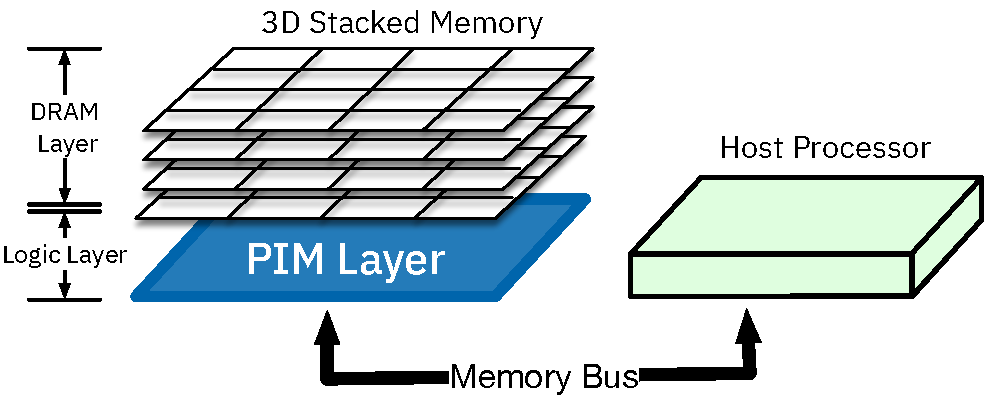
\includegraphics[width=0.80\columnwidth ]{figures/pim.pdf}
    \caption{Processing-In-Memory layer in 3D-stacked memory.}
    \label{fig:pim}
\end{figure}


\subsubsection{PIM hardware architectures.}
The progress made in 3D-stacked memory technology enabled embedding of logics or even processors into memory. Two of the most prominent example of 3D-stacked memory are \emph{Hybrid memory cube (HMC)}~\cite{hmc}, and \emph{High Bandwidth Memory (HBM)} \cite{amd-hbm,samsung-pim}. \autoref{fig:pim} demonstrates the architecture of 3D-stacked memory and the PIM layer. Stacked memory architectures vertically stack DRAM layers on top of each other and connect the vertical partitions of memory using high-bandwidth through-silicon vias (TSVs). A typical 3D-stacked memory configuration can employ thousands of TSVs \cite{primer-on-pim}, which makes its internal memory bandwidth far exceed that of traditional memory systems. At the bottom of the memory stacks, there is a \emph{PIM layer}, or logic layer, that can host hardware logic that can interact with both the host processor and the DRAM memory. The PIM layer can be special-purpose hardware logic~\cite{invisimem,prime} that is embedded into the memory chip, or a general-purpose processor~\cite{upmem,samsung-pim,smcsim,pim-architecture} that runs software called the \emph{PIM kernels}, analogous to the kernels loaded onto GPUs. Most 3D-stacked PIM architecture requires changes to the host-side processor~\cite{pim-architecture}, but PIM architectures that can integrate with commodity processors also exist~\cite{upmem,upmem-atc,pim-architecture}. UPMEM~\cite{upmem} introduced its PIM architecture on a traditional DRAM chip. Lee et al.~\cite{pim-architecture} designed and implemented a generalized PIM architecture and programming model to support PIM-accelerated DNN computation on HBM memory. Both of these prototypes have real hardware implementations and are compatible with off-the-shelf systems~\cite{upmem-atc,pim-architecture}.

%\hdr{Using PIM for security.} There have been works that harness PIM computation for security purposes. InvisiMem \cite{invisimem} and ObfusMem \cite{obfusmem} proposed enhancing the host-side memory controller and the memory-side memory controller with capabilities to form an encrypted communication channel that also encrypts the accessed address and type of operation (read or write). In doing so, the systems can provide security guarantees similar to Oblivious RAM (ORAM) without significant performance overhead~\cite{obfusmem,invisimem}. Other works demonstrated that PIM is beneficial for accelerating security operations \cite{sdimm, near-data-security, hega}. \cite{near-data-security} suggests delegating Bonsai Merkle Tree memory authentication operations to memory. Secure DIMM (SDIMM)~\cite{sdimm} offloads that a part of the ORAM access routine to logic inside a DIMM memory to reduce the bandwidth usage of ORAM algorithms. In \cite{hega}, the authors propose HEGA, a PIM architecture that accelerates homomorphic encryption search. All of those researches show that PIM can significantly reduce the memory bandwidth of memory-intensive security applications.
% \hdr{Acceleration of security operations.}




\newcommand{\goal}[1]{\hyperref[g#1]{O#1}}

\subsection{Confidential Computing in Cloud and Challenges}
\label{subsec:confidential}

Supporting confidential computing in the untrusted cloud is a common goal shared by the industry and academia, as evidenced by confidential computing services being offered by cloud service providers \cite{azure,google-confidential-computing,nitro}. 

% Several works have proposed various SGX-based confidential computation schemes. The works explored the design space in using Intel SGX for secure data computation in the cloud~\cite{vc3,enclavedb,occulemency}. VC3~\cite{vc3} proposes an architecture for performing distributed MapReduce in the untrusted cloud, in which sensitive code and data are protected. EnclaveDB~\cite{enclavedb} protects the database and the querying process using SGX. Occlumency~\cite{occulemency} proposes an SGX-based deep learning inference that ensures confidentiality and integrity of user data. 
\subsubsection{Secure enclaves and the cloud. }
Modern processor architectures support secure enclaves for isolated execution of sensitive code and data. Intel SGX~\cite{sgx} is the most commonly available secure enclave in the cloud. SGX provides protected memory pages called \emph{Enclave Page Cache (EPC)} in which the sensitive subset of a program and processed data can be protected. Memory accesses from the processor to the EPC region are automatically encrypted on the memory bus by the memory encryption engine~\cite{sgx-explained}. A remote user can verify the integrity of a deployed enclave through \emph{remote attestation}, a procedure that allows an enclave to \emph{attest} its code and data with a measurement, signed by a secure hardware cryptographic key. 

\subsubsection{Memory limitations of secure enclaves.} 
The limited memory capacity is one of the main factors that hinder the adoption of SGX-based secure enclaves. SGX has a limited EPC capacity of 128MB; large data computation has to be broken down into smaller batches~\cite{occulemency,bigmatrix}. DNN model-based inference frameworks that are aware of and optimized for the SGX's memory limitations are also proposed~\cite{occulemency,kim2020vessels}. Moreover, it is shown that EPC page swapping is expensive when a large amount of secure memory is used~\cite{zerotrace,scone} (up to $1000\times$ performance overhead). Designs for external secure storage devices for secure enclaves are also explored by several works to complement SGX's memory limitation~\cite{trustore,invisimem,obfusmem}.


\subsubsection{Side-channel attacks on enclaves.}
Researchers have shown that secure enclaves can fall vulnerable to side-channel attacks. The microarchitectural side-channels and the data access pattern captured on the memory bus are shown to be exploitable against SGX secure enclaves to undermine the confidentiality of the computed data~\cite{leaky-cauldron,sgx-cache-attack,sgx-grand-exposure,membuster}. Microarchitectural side-channel attacks exploit \emph{microarchitectural resources sharing} to extract sensitive information about the enclave execution~\cite{sgx-cache-attack,sgx-grand-exposure}. For instance, attackers can infer secret-dependent cache lines accesses of an enclave based on the cache timing~\cite{sgx-grand-exposure}. On the other hand, even though memory requests from an enclave are encrypted, the \emph{access pattern} of data can also leak secrets. Membuster~\cite{membuster} demonstrated an attack that uses a capturing device attached to the memory bus that extracts sensitive information only from the \emph{addresses side-channel} of SGX enclaves.

% \hdr{Approaches for side-channel elimination.} 
% The causes for most memory side-channels are the differences in the memory access pattern that depends on the secret input~\cite{raccoon}. Program obfuscation and oblivious RAM (ORAM) adaptations inside enclave~\cite{raccoon,zerotrace,obfuscuro} are the generally accepted solutions for memory side channels. Program obfuscation transforms potentially unsafe programs into side-channel-free programs~\cite{raccoon,obfuscuro,ghostrider}, while the use of ORAM algorithms hide the access pattern to sensitive data structures~\cite{raccoon,obfuscuro,zerotrace,ghostrider}. However, due to the high performance overhead, those approaches are often inapt for data-intensive computing.

% \new{
% Alternatively, there are also approaches that help eliminate side-channels from software, by providing ORAM-like obliviousness with trusted hardware~\cite{trustore,obfusmem,invisimem}. Obfusmem~\cite{obfusmem} and Invisimem~\cite{invisimem} construct a secure channel between the host CPU's memory controller and the memory-side memory controller to hide the memory access pattern. Trustore~\cite{trustore} uses a narrow single-channel to interface a PCIe storage and SGX enclave to mitigate side-channels in processor caches and address side-channel on the bus. }

\subsubsection{Extending trust to the peripheral devices.}
Since achieving trusted I/O with a device is not viable in SGX's security model, the device itself must actively participate in establishing a secure channel with the processor enclave. Existing works have presented peripheral device designs that create a secure communication channel with the host enclaves. Graviton~\cite{graviton} proposed a set of hardware modifications for GPUs that enables secure acceleration for confidential computing in the cloud. HIX~\cite{hix} sought to achieve the same goal but proposed modifications to the I/O interconnect between CPU and GPU. Trustore~\cite{trustore} uses an FPGA storage device to provide extra storage space that is free of memory side-channels for SGX. One design component these works have in common is remote attestation and secure communication channels. Our design, \thename, adapts many of the requirements for a device in extending processor enclave's trust to I/O devices generalized by the previous works.  

\subsection{Mitigations of Access Pattern Side-channels}
\label{subsec:oram}
Oblivious RAM (ORAM)~\cite{path-oram,ring-oram,freecursive-oram} is accepted as a general mitigation for the access pattern side-channels. ORAM algorithms transform the original data accesses into sequences of obfuscated accesses that seem random to attackers~\cite{ring-oram}. There have been adaptations of ORAM to SGX enclaves~\cite{zerotrace,obfuscuro} to hide the enclave's access patterns to sensitive data structures. Secure processor prototypes that integrate ORAM logic into the memory controller also exists~\cite{freecursive-oram,ascend} that hides the access pattern on the bus. However, the performance overhead of ORAM-based approaches may deter their adaption~\cite{zerotrace}. In response, alternative approaches are proposed that build an encrypted channel between the user and secure storage. Invisimem~\cite{invisimem} and Obfusmem~\cite{obfusmem} introduced encryption capabilities to the CPU-side and the memory-side controllers to encrypt the entire memory request, including the \emph{accessed address} and \emph{type of operation}, to achieve ORAM-like security guarantees. Trustore~\cite{trustore} employed the same technique to hide the address-based side-channel by establishing an encrypted channel between an SGX enclave and the secure FPGA-based storage. 

\section{SE-PIM Objectives and Challenges}
In this section, we first establish the design objectives of \thename. We then explain the generalized baseline PIM architecture, on which \thename's design proposals construct confidential computing capabilities. Against the threat model, which is also explained in this section, we explain the unique challenges that our design must mitigate. 


% describe the threat model in \cref{subsec:threat-model}. 
% We describe a generalization of PIM architectures, which we refer to as \baseline (\cref{subsec:pim-baseline}).

% Then, we illustrate the challenges in achieving our objectives, even the design additions to \baseline for confidential computation in~\cref{subsec:challenges}.


\subsection{Design Objectives of SE-PIM}
\label{subsec:objectives}
Our goal is to enable the memory to actively cooperate with a CPU-based enclave to perform confidential computation. Hence, our system functions as a secure memory extension for the host enclave and a secure accelerator for data-intensive computation. We identify the high-level objectives for \thename as follows. 

\hdr{\thename is a trusted memory extension.} \label{g2} 
One of the \thename's objectives is to function as a secure memory extension that supplements the limited memory capabilities of secure enclaves. The memory limitation of secure enclaves is a substantial problem that impedes the widespread adoption of confidential computing for large data. Many works proposed partitioning large data into batches that fit into the enclave memory space, but at the cost of performance~\cite{bigmatrix,occulemency}. On the other hand, turning memory into an active entity in secure data storage and processing can solve the problem of limited memory space in cloud enclaves. 



\hdr{\thename is a secure large data computation accelerator.} \label{g3} 
PIM-enabled memory devices are on the horizon~\cite{samsung-pim,amd-hbm,upmem,pim-architecture} and their advantages in accelerating data-intensive cloud workloads have been demonstrated~\cite{upmem-atc,upmem-benchmark,scalable-pim-acc,nda,pim-architecture}. Our objective is to take advantage of the processing capability of PIM by allowing the host enclaves to launch a protected PIM kernel on \thename-enabled memory banks. Furthermore, our hardware modifications must not introduce significant overhead to PIM computation.
 
We observe that PIM can inherently reduce the attack surface to many side-channel attacks that have been an existential threat to many processor enclaves~\cite{sgx-cache-attack,leaky-cauldron,sgx-page-table}. Performing computations where the data resides eliminates side-channels that occur while the data moves in a route on the memory bus or stored in shared storage, such as the processor caches~\cite{sgx-cache-attack}. We observe that such \emph{zero-copy} data transfer in PIM-assisted computations eliminates \emph{runtime} data movement between the CPU and PIM, thereby inherently minimizing the address side-channels on the memory bus~\cite{drama,membuster}. 

% However, as we illustrate in \cref{subsec:challenges}, there can be subtle side-channels incurred from the \emph{memory content change} that can leak sensitive information about the PIM kernel execution. 


% We carefully analyze the attack vectors when designing \thename as a secure memory extension. We explain in \cref{subsec:challenges} that simply encrypting the memory content is insufficient against the attack vectors that exploit the data \emph{access pattern} to leak information. We also show that memory integrity is not fully protected even with authenticated encryption such as AES-GCM.

% \hdr{Security objectives and scope.} 
% \thename provides a secure computation offloading model between a processor enclave and a \thename-enabled memory module. A secure connection with the processor enclave is established through remote attestation. We protect the integrity and confidentiality of the data used by \thename and the host enclave. We also guarantee the elimination of observable access patterns to the in-\thename data from both the CPU-side enclave and \thename units in each bank. We only trust the \thename units which include our hardware modifications, and CPU-based enclaves. Other software and hardware components in the system are distrusted. Side-channel attacks on the host CPU that take advantage of microarchitectural characteristics are out of the scope of our protection. The host enclave can offload sensitive operations to \thename units to reduce the attack surface. We also consider the electromagnetic side-channel and power side-channel of \thename out-of-scope~\cite{power-side-channel-accelerator}. The row hammer attacks are also not considered.

% \hdr{Attacker capabilities.}
% The primary objective of the adversaries is to extract sensitive information protected by secure enclaves through powerful attacks that they can launch with kernel privilege and physical access. As the privileged software manages the memory mapping, a malicious system software could map a region of physical memory into its own memory space or to a malicious process memory space. This also allows the attacker to passively or actively tap into every I/O communication with DMA buffers of MMIO from the host with the PIM device. 

% With physical and privileged software accesses to the system, an attacker can perform physical attacks on the MMIO interface of devices and the memory system. The attacker might corrupt the packet by tampering with the payload. They might also replay or delay a previously valid packet on the bus. The attacker could perform access pattern analysis to infer sensitive information from the memory accesses or MMIO packets \cite{access-pattern-disclosure,membuster}. We also consider \emph{DMA attacks} \cite{write-access-pattern}, where an attacker takes snapshots of the memory content at a high frequency to extract the changes in memory. \emph{Cold boot} attacks, where an attacker exploits the memory retention behavior of DRAM to extract the content of memory directly, are also considered~\cite{coldboot-attack}. 

\subsection{Baseline PIM}   
Prior to explaining the challenges in retrofitting a PIM architecture to have confidential computing capabilities, we first explain a generalized PIM architecture without support for confidential computing and its programming model, named \baseline. Using the \baseline architecture, we explain the challenges in \thename's imperative additions to \baseline for confidential computing.

\hdr{\baseline architecture.} Our baseline PIM model (\baseline) is a generalization of several works that introduces compute capabilities to memory~\cite{upmem-atc,tesseract}. We assume that in each memory bank of a memory module (e.g., 3D-stacked memory or DIMM memory stick), there is an integration of a programmable processing core (i.e., the \emph{PIM core}). The PIM cores can execute PIM kernels, program binaries compiled to run on a PIM core. As to the processing capacity of these processors, they often lack processor caches~\cite{upmem,smcsim,top-pim,neural-network-training}, and packaged with a low-latency on-chip memory, or \emph{PIM local memory}~\cite{smcsim,upmem,cho2020accelerating}. The local memory stores the PIM kernel and data a PIM core operates on. The PIM core accesses data inside a memory bank thorough \emph{direct memory access} (DMA). It requests the on-chip DMA engine to fetch batches of data into its local memory and process the data there. We do not assume architectural support for cache coherency between the PIM core and the host processor. A cache coherence scheme often requires PIM-aware changes to the host processor architectures~\cite{pei,conda}. Therefore, our current design does not involve concurrent computation on the same data between the PIM core and host processor.


\label{subsec:pim-baseline}
\begin{figure}[t]
    \centering
    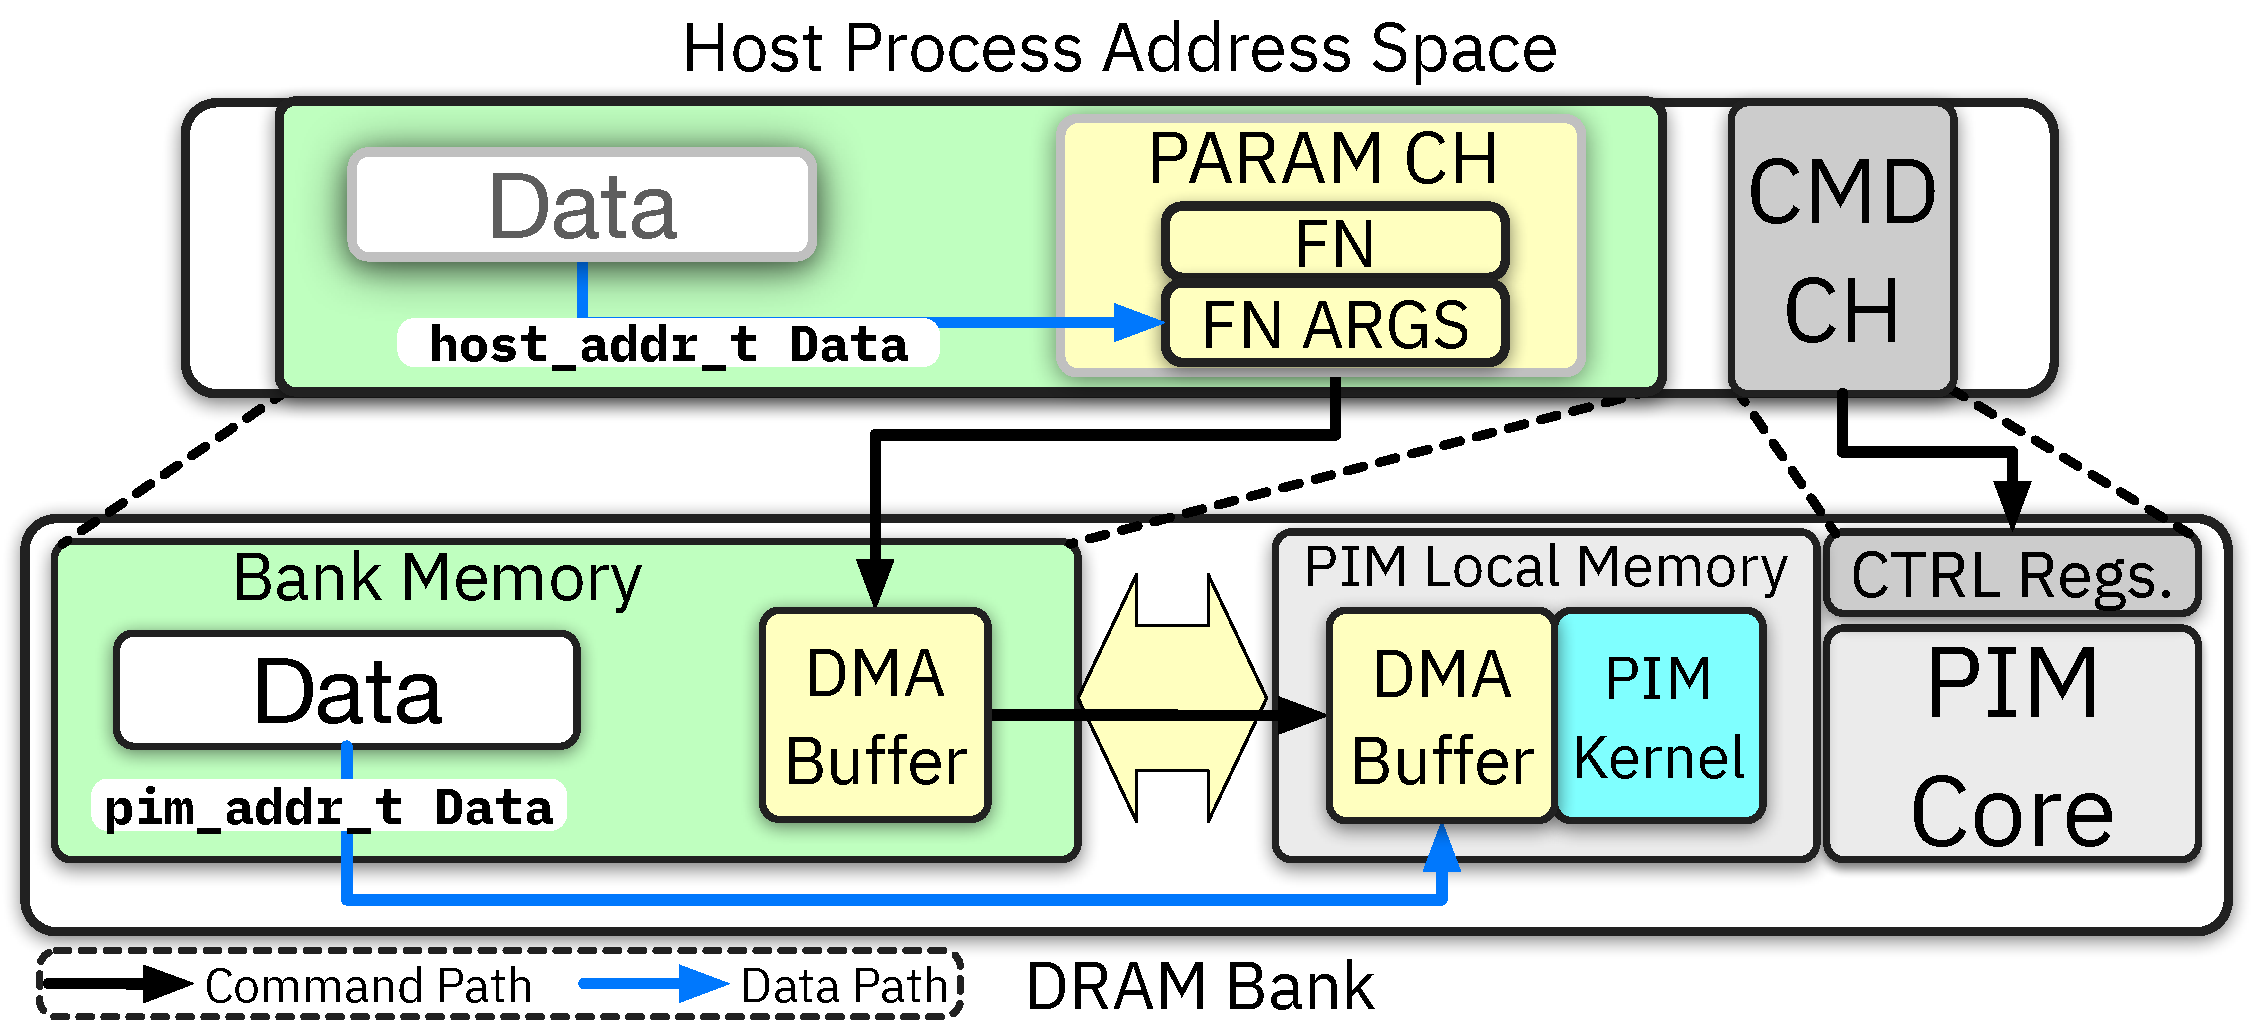
\includegraphics[width=.9\columnwidth]{figures/sepim/interfaces.pdf}
    \caption{The communication interfaces between the host and PIM using mappings of memory in host process address space.}
    \label{fig:interfaces}
\end{figure}

\hdr{Host-side access to memory.}
The memory bank of \baseline can be used as the normal memory space for the host program. We assume a direct mapping approach for data transfer between the host process and PIM-enabled memory banks; the physical address space of the memory bank is mapped by the driver into a contiguous address range in the host process (demonstrated in \autoref{fig:interfaces}). The CPU uses the mapped addresses to transfer data into the memory bank directly (the \emph{data channel}). We assume an uncached mapping for the PIM memory banks for data coherency between the host CPU and PIM such that the memory modifications in the host are immediately visible to PIM. \baseline must also support address translation on the PIM core, because the host and PIM uses different address spaces. To achieve this, the PIM core and the host process share a contiguous memory range with a direct mapping scheme, a common design seen in PIM designs~\cite{tesseract}. The PIM core can obtain the in-bank physical address from the host virtual address through a constant offset (\texttt{pim\_addr} $=$ \texttt{host\_addr} $-$ \texttt{C}), for all shared addresses. 

\hdr{Interfaces between host and PIM.}
A host program is typically employed to control the execution of the PIM cores. Similar to most I/O devices, the host process and \baseline communicate using two interfaces, MMIO registers, and DMA. For MMIO-based communications, the PIM system exposes registers to the host, which are used to send \emph{commands} to the PIM units to control their execution. We refer to this as the \emph{command channel} (CMD CH in \autoref{fig:interfaces}). DMA-based communication in \baseline copies data within the memory bank into PIM local memory using the fast PIM bus close to the memory. Hence, PIM-based DMA is different from the DMA communication of other devices that requires data to move across the slow peripheral buses. The host uses the DMA buffer to send \emph{parameters}, a data structure containing arguments for the PIM kernel (e.g., pointers to data inside memory) and commands. We refer to this channel for communication as the \emph{parameter channel} (PARAM CH in \autoref{fig:interfaces}). In order to utilize PIM, the host program loads the PIM kernel into PIM local memory (typically via MMIO~\cite{upmem-atc,smcsim}), writes the parameters that have the function name and its arguments into the parameter channel, and sends a command to the command channel to start executing the PIM kernel. The PIM core then fetches the parameters into its local memory and executes the requested function with the arguments.

\hdr{Zero-copy data exchange.} PIM computations typically utilize \emph{zero-copy} data exchanges. As demonstrated in \autoref{fig:interfaces}, the PIM kernel takes \emph{pointers} to data already located within memory as the arguments for execution. The PIM kernel uses the pointers as the source address to fetch data into the local memory for processing with efficient DMA transfers. With zero-copy, data exchanges on the slow memory bus are reduced, and efficiency is achieved in terms of bandwidth utilization and CPU cycles~\cite{pointer-chasing,smcsim,primer-on-pim}.


\subsection{Threat Model}
\label{subsec:threat-model}
%\hjc{check}
We protect the integrity and confidentiality of the data used by \thename and the host enclave. We also guarantee the elimination of observable access patterns to the in-\thename data on the memory bus. We only trust the \thename-enabled memory that contains our hardware modifications and CPU-based enclaves. Other software and hardware components in the system (e.g., the OS and other applications) are distrusted. Side-channel attacks on the host CPU that take advantage of microarchitectural characteristics are out of our protection scope. The host enclave can offload sensitive operations to \thename units to reduce the attack surface. We also consider the electromagnetic side-channel and power side-channel of \thename out-of-scope~\cite{power-side-channel-accelerator}. The row hammer attacks are also not considered.

%\hjc{Explain the trusted components }
Regarding the security of the PIM itself, we assume that the tightly integrated PIM-enabled memory bank, which includes the PIM core, PIM local memory, and our introduced modifications, are secure from physical attacks. The connections inside the PIM hardware are often connected with highly integrated connections (e.g., Silicon Vias (TSV)), so we assume that using hardware probes to snoop data contents from PIM is infeasible.




\subsection{Challenges}
\label{subsec:limitations}
\label{subsec:attack-vectors}
\label{subsec:challenges}
% In this section, we illustrate the challenges in achieving our objectives depicted in \cref{sec:goals}. 

%We elaborate the assumptions we make on the baseline PIM to enable confidential computation. Then,  (described in \autoref{fig:attack-vectors}).

PIM exhibits many inherent strengths as a side-channel resistant confidential computing accelerator for host enclaves. However, the required design changes for PIM architectures have not been explored to the best of our knowledge. Our contribution lies in identifying the unique challenges and proposing a set of design changes for mitigating them.

We start by introducing rudimentary features that are essential for confidential computation into the aforementioned \baseline. Namely, we assume that the attestation and secure channel establishment capabilities are now in place, similar to previously proposed secure hardware accelerator architectures~\cite{graviton,trustore,invisimem}. This means that both parties -- the host enclave and PIM -- communicate through encrypted channels to exchange commands and data. The encrypted data is stored in the memory banks and only to be decrypted inside PIM local memory when the PIM core proceeds to process the data.

However, we see that there still remains critical challenges in securing the workload computation performed in cooperation of the host enclave and PIM. We rigorously inspect all attack vectors that may allow the adversary to leak information about the \thename-assisted confidential computation. \autoref{fig:attack-vectors} summarizes the challenges that we identify. In the rest of this section, we explain the challenges in depth.

% We point out an inherent performance limitation in the baseline PIM in achieving end-to-end encryption with the host enclave and illustrate our point with an evaluation of real PIM hardware. In addition, we observe the attack vectors that must be mitigated for a PIM to function as secure storage and accelerator. The attack vectors are illustrated in \autoref{fig:attack-vectors}.

%\autoref{fig:attack-vectors} displays the security challenges in \baseline that we must address in the design. 



\begin{figure}[h]
    \centering
    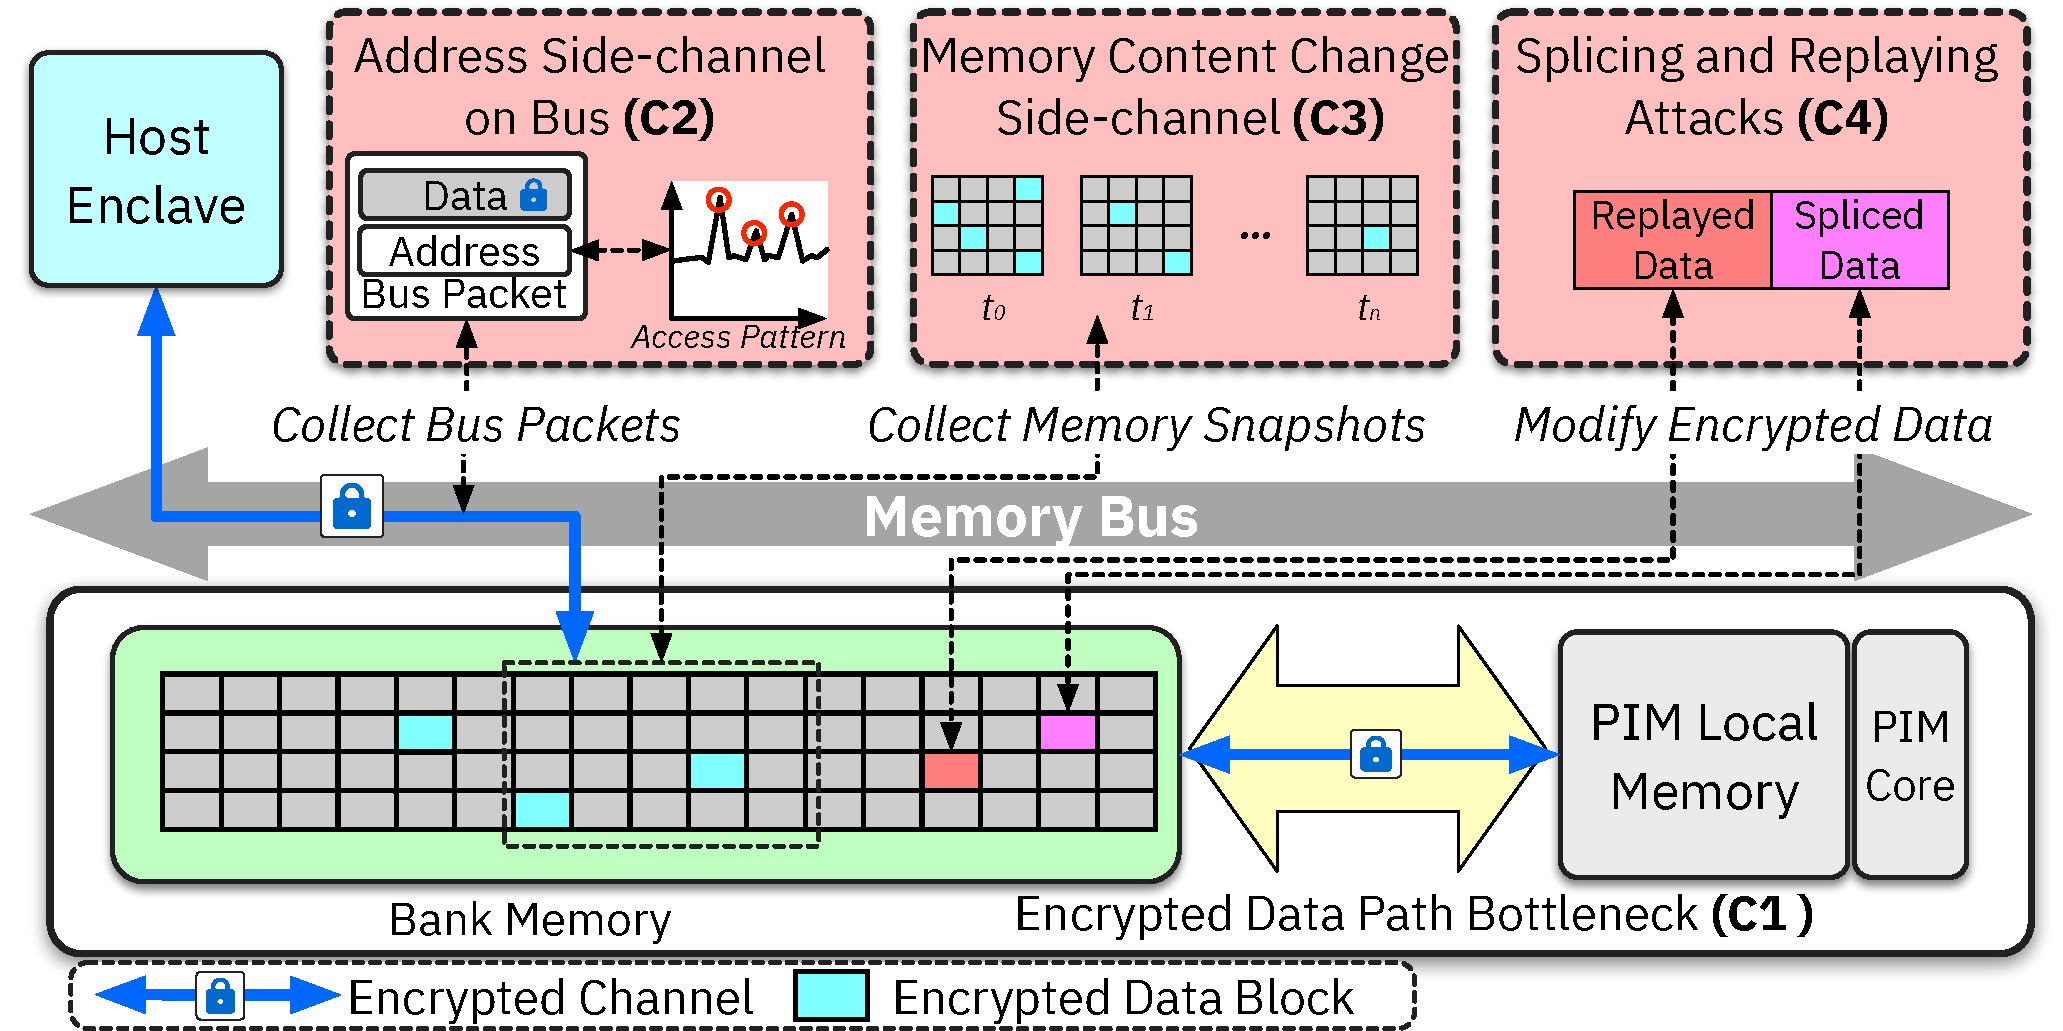
\includegraphics[width=0.8\textwidth]{figures/sepim/attack-vectors.pdf}
    \caption{Challenges faced by \baseline. Encrypted data movement between PIM local memory and the bank memory creates a performance bottleneck (C1). Memory accesses by the host enclave can leak the \emph{accessed address} on the bus (C2). An adversary can also monitor the memory content changes by quickly taking memory snapshots and comparing the differences (C3). Data inside memory is also vulnerable to splicing and replay attacks (C4).}
    \label{fig:attack-vectors}
\end{figure}
\begin{figure}[h]
    \centering
    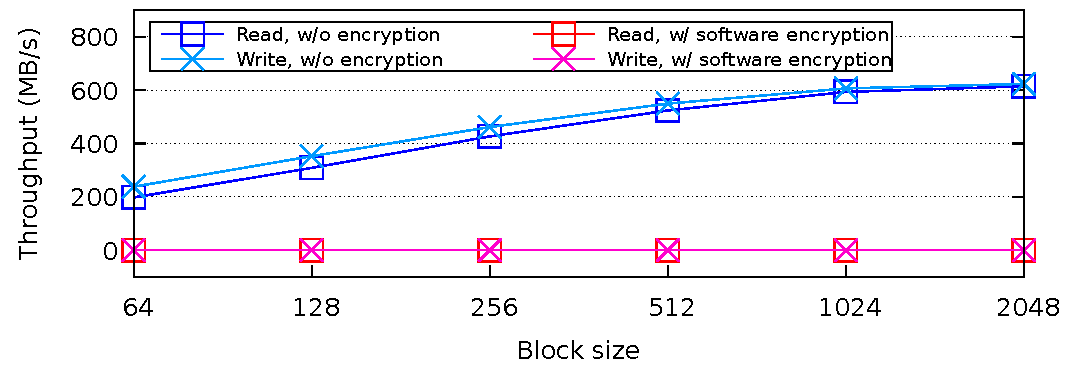
\includegraphics[width=.8\columnwidth]{figures/sepim/upmem-bandwidth.pdf}
    \caption{The memory throughput with and without software AES encryption on UPMEM PIM hardware.}
    \label{fig:upmem-aes}
\end{figure}



\newcommand{\challenge}[1]{\hyperref[c#1]{C#1}}

\newcommand{\attack}[1]{\hyperref[a#1]{A#1}}
\textbf{C1: Performance overhead of end-to-end encryption.}\label{c1}
It is essential that the command and data channels between the host and core are encapsulated with an end-to-end encrypted channel. However, we found that this is infeasible without hardware acceleration for encryption. To support our point, we evaluated the performance of working with encrypted data using software-based AES using \emph{mbedtls} on UPMEM’s real PIM hardware~\cite{upmem,upmem-atc}. The performance of encrypted DMA transfers is measured in both ways; the PIM core encrypts the data before transferring it from its local memory to the memory bank and decrypts the data as the data comes in the reverse direction. We measured the latency of each transfer from the initiation of encryption/decryption to the completion of the DMA transfer. 

As shown in \autoref{fig:upmem-aes}, software AES incurs immense performance overhead. The throughput plummeted from 600 MB/s to 0.5 MB/s, around 1200$\times$ lower throughput for both read and write. The results convinced us that hardware acceleration for symmetric key cryptography must be included for confidential computing in PIM design. Unlike convention accelerators (e.g., GPU), PIM designs have more constraints in terms of power and area constraints, which will always be limiting factors in PIM designs~\cite{amd-hbm,hmc,upmem-atc}. 
 
%PIM excels at memory-intensive HMC and HBM~\cite{hmc,amd-hbm}, and the power and area constraints 

\textbf{C2: Address side-channel on memory bus.} \label{c2}
We observe that when the host access PIM memory banks by writing to the memory mappings of \baseline, an attacker can capture the accessed physical addresses on the memory bus with a snooping device. The attack vector was shown exploitable even on SGX secure enclave, where the memory content is encrypted~\cite{membuster}. Although sequential data placement into the memory bank does not generate observable access patterns, host-side data accesses that are parts of the data processing computation can leak sensitive information about protected data. 
%or instance, the host application might retrieve or update a specific data block in the memory bank, which leaks differentiable patterns on the memory bus.% The elimination of such side-channel is necessary to satisfy the design objective \goal{2}. 

%\hjc{Accessing encrypted data is a challenge? from whose perspective?}
\textbf{C3: Side-channels from memory content changes.} \label{c3}
In \baseline, the memory bank mapping is managed by the kernel, which is untrusted in the threat model of secure enclaves. The untrusted kernel can directly access the memory content of \baseline through the memory mapping or map the bank memory into a malicious process's address space. On the other hand, an attacker-controller DMA device on the same system can also access the bank's content. Even though data inside the bank can be encrypted, an attacker can take snapshots of the memory and extract the changes in the memory content made by the PIM kernel. Due to the limited size of the PIM’s local memory, the PIM kernel must work with the encrypted data in batches, which is not necessarily sequential. A batch of data will be fetched from the memory bank to be decrypted and processed. Then, depending on the PIM kernel logic, the memory content might be updated with new values. Such operations may inadvertently create recognizable patterns in the eyes of the passive adversary. Research has shown that by only observing the memory change over time, attackers can recover sensitive information about the unencrypted data~\cite{write-access-pattern}. %This side-channel contradicts our design objective of enabling \thename as a secure accelerator (\goal{3}) by leaking information about the execution of the PIM kernel.


\textbf{C4: Providing protection against splicing and replaying attacks.} \label{c4}
With the same methods described in \challenge{3}, attackers can also modify the content of \baseline's memory banks.
Encrypting data with authenticated encryption algorithms (e.g., AES-GCM) protects encrypted data against direct tampering by attaching an authentication tag to the encrypted data. However, data inside memory is susceptible to \emph{splicing} and \emph{replaying} attacks when external entities modify the encrypted data. The splicing attack replaces data from one location with a valid encrypted data block from another location. The replaying attack reverts a chunk of encrypted data to a previously valid state. Both attacks trick the integrity checking of authenticated encryption algorithms into verifying that maliciously crafted data blocks have not been tampered with. Compromising data integrity might also affect the correct execution of the PIM kernel; PIM might use outdated data or data from an incorrect location for processing. Hence, the attacks jeopardize the objectives of \thename both as a secure memory extension and a secure accelerator. The mitigation of replaying and splicing attacks typically requires additional metadata storage (e.g., the latest timestamp of each data block) and additional verification procedures that would inadvertently introduce overheads to each memory access~\cite{bonsaimerkletree,common-counter}. 


% Objectives / Challenges
% SE-PIM Architecture --> Hardware Stuff
% -- Remote attestation and Secure channel (Short)
% -- Hardware acceleration for encrypted data flow
% -- Preventing side-channels during computation
%    -- Controlled access channel
%    -- DRAM lockdown 
%       -- gives PIM core control over DRAM access control
% -- 
% Programming Model
% -- 
% Implemenation 
% Evaluation
% Discussion
% Related Work
% Conclusion




\section{SE-PIM Architecture}
\label{sec:design}
The design of \thename specifically mitigates the challenges explained in the previous section. Our design brings imperative changes for \baseline to overcome the unique challenges in achieving its objectives. We explain each architectural change and how they mitigate the challenges in this section. 


% \cref{subsec:hardware} illustrates the overview of \thename architecture.  We explain remote attestation and secure channel establishment in \cref{subsec:attestation}. \cref{subsec:aes-dma} illustrates our design for encrypted data flow acceleration, addressing \challenge{1}. \cref{subsec:side-channels} elaborates how we address the challenges \challenge{2}, \challenge{3} and \challenge{4} with the introduction of DRAM lockdown and the controlled access channel.


% In \cref{subsec:access-control}, we describe the DRAM lockdown logic, which addresses \challenge{3} and \challenge{4} . Our secure memory access interface in \cref{subsec:secure-access} allows the host enclave to hide its memory access pattern, which solves \challenge{2}. Finally, to deal with \challenge{1}, we introduce AES acceleration to the DMA engine to efficiently transfer encrypted data between PIM local memory and the memory bank (\cref{subsec:aes-dma}).


\begin{figure}[t]
    \centering
    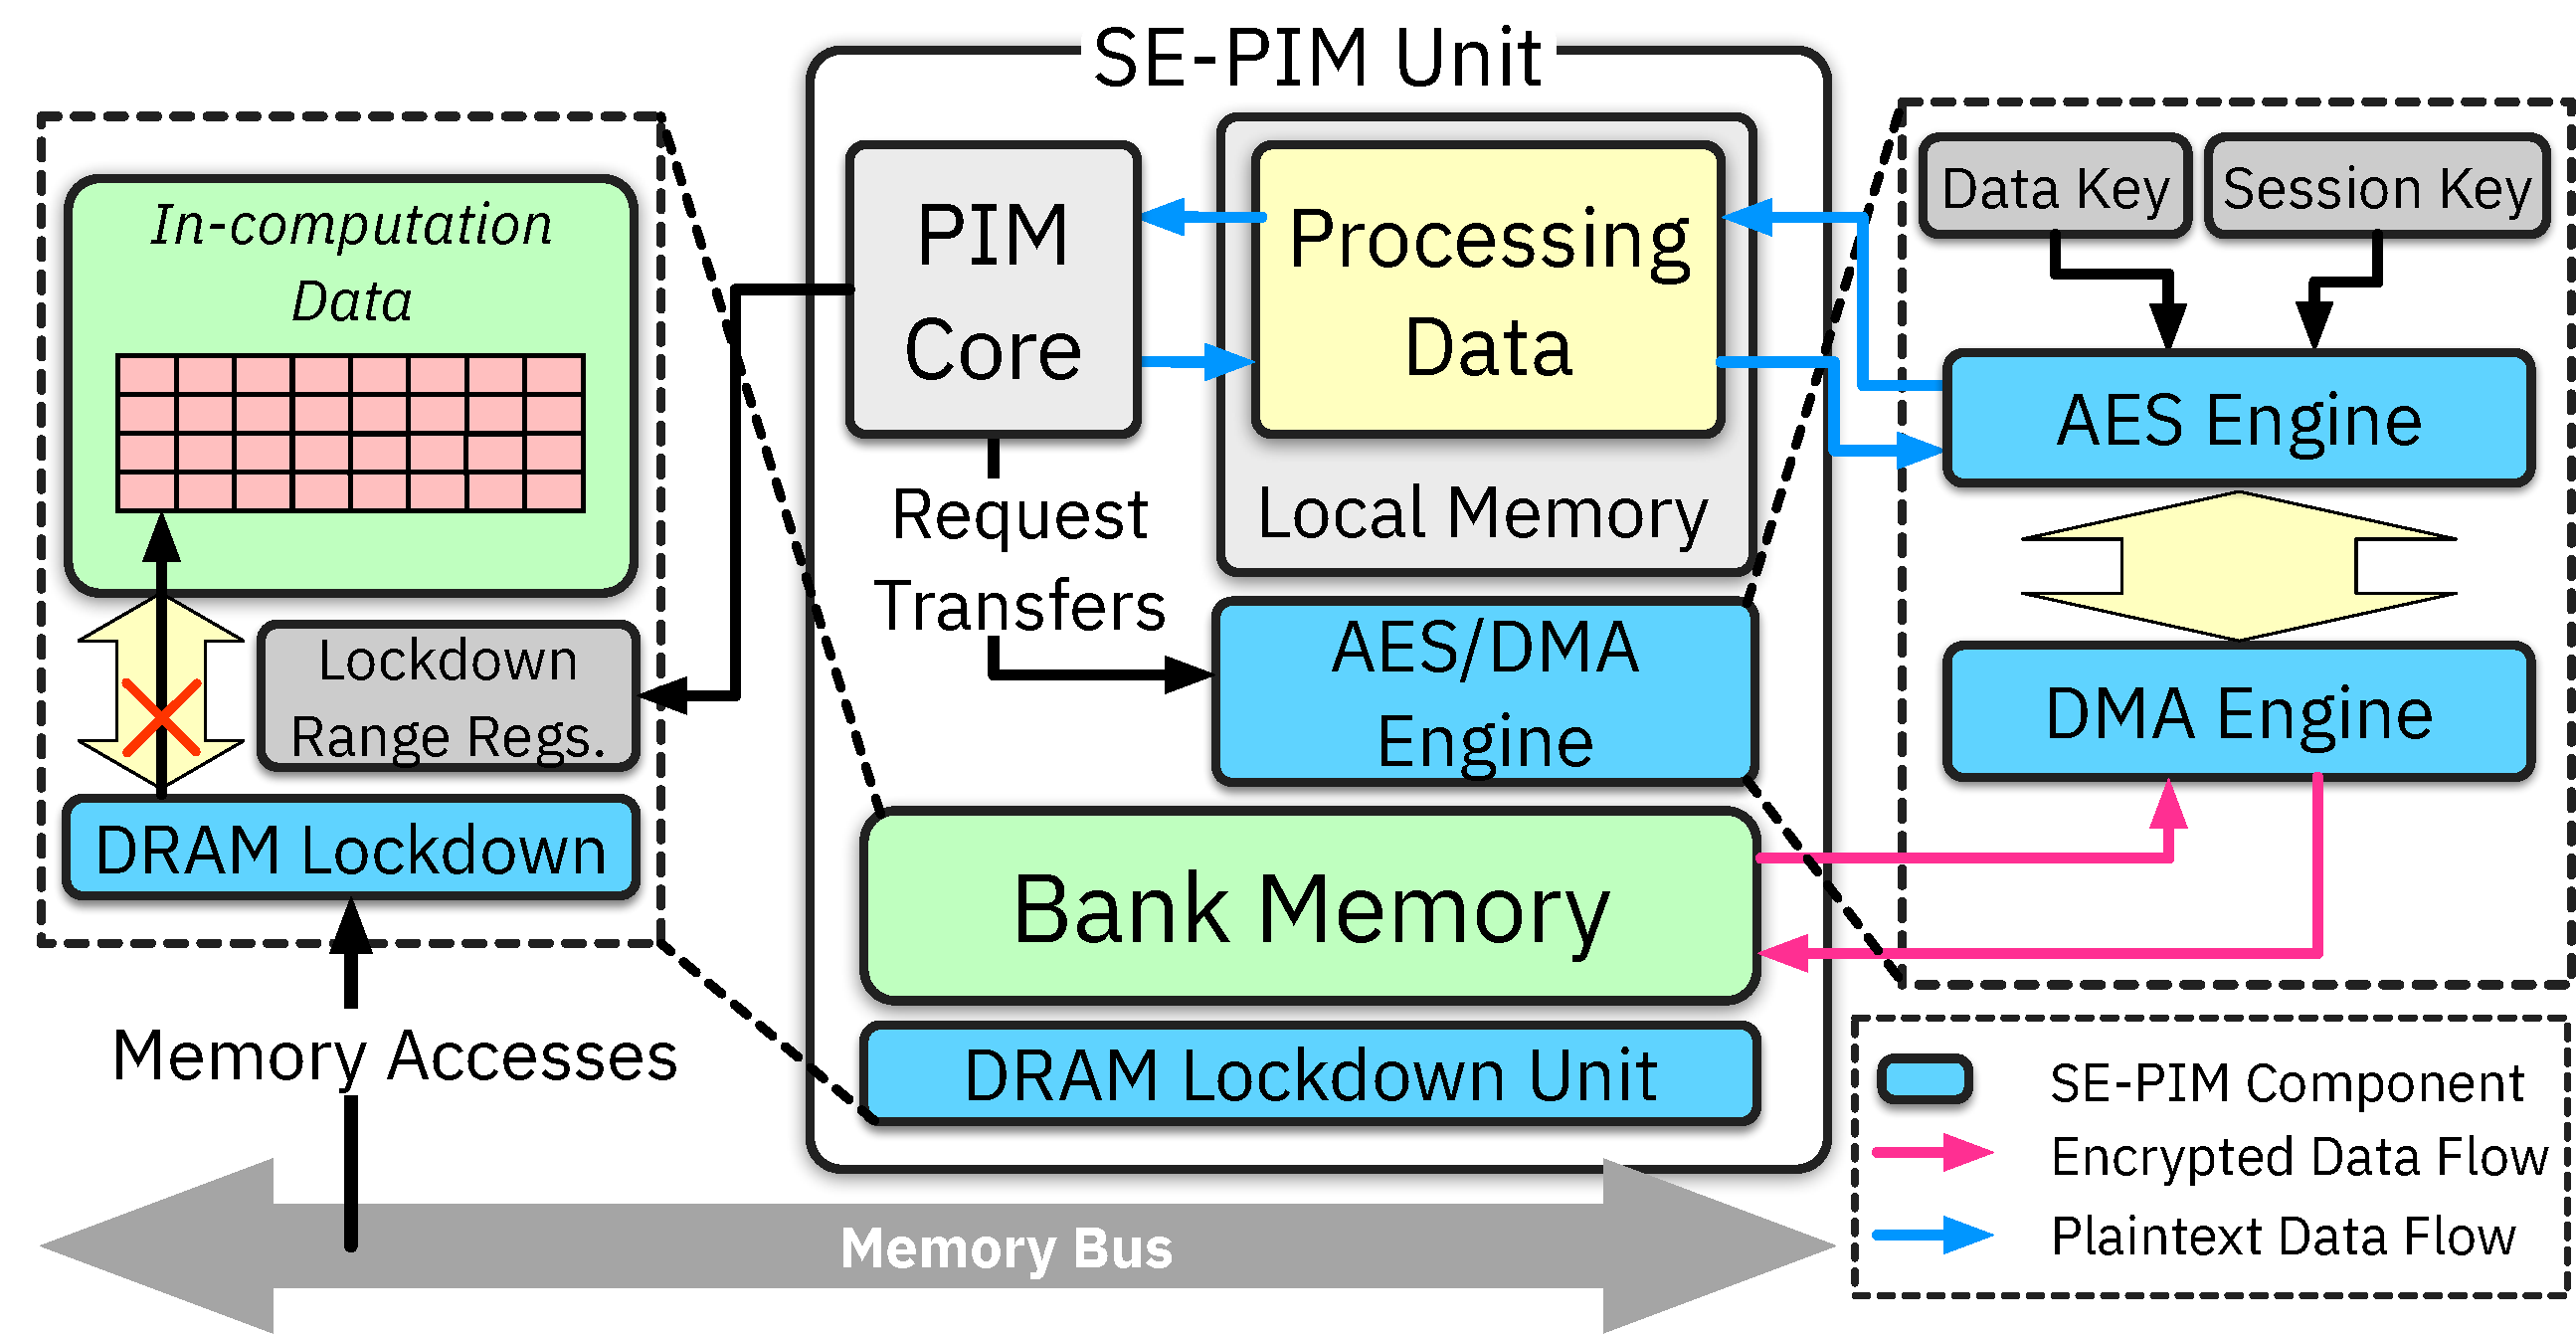
\includegraphics[width=.90\columnwidth]{figures/sepim/components.pdf}
    \caption{Overview of \thename hardware architecture.} 
    \label{fig:overview}
\end{figure}

\subsection{Overview}
\label{subsec:hardware}

% Internal
\autoref{fig:overview} shows the \thename architecture. \thename hardware design contains modifications to the \baseline architecture mentioned in \cref{subsec:pim-baseline} to protect the confidentiality and integrity of in-memory computations.
In \thename, the memory banks serve as a conventional main memory for the host and storage for encrypted data during confidential computing. A \emph{\thename unit} is included in each memory bank. Each \thename unit is equipped with a PIM core, PIM local memory, \emph{DMA/AES engine} and \emph{DRAM lockdown unit}. The functions of the PIM core and local memory are similar to that of \baseline. The AES/DMA engine introduces hardware acceleration to the DMA engine that significantly accelerates encrypted data transfers. The DRAM lockdown unit enforces \emph{DRAM lockdown}, a mechanism that prevents unauthorized access into the protected data during confidential computation. The DMA/AES engine and DRAM lockdown unit are hardware modules controlled by the PIM core running \thename kernel through MMIO registers. ROM and key storage are also introduced that can be used by all \thename units within a memory module. ROM includes cryptographic primitives (e.g., key pair generation, key signing) and preprogrammed procedures (e.g., attestation) that serve the \emph{commands}. The key storage contains the root endorsement key (EK), the root of trust to enable remote attestation. 

%The host enclave communicates with \thename through two interfaces, an in-memory DMA buffer and MMIO registers. 

We will further elaborate how a host enclave uses \thename through our programming model in \cref{sec:prog-model}. \emph{\thename components} in \autoref{fig:overview} (DMA/AES engine, DRAM lockdown unit) are the new hardware components that we introduce to enable confidential computing acceleration. We will explain the necessity and functionalities of the remaining components in the following subsections. 
 

\subsection{Remote Attestation and Secure Communication Channel} 
\label{subsec:attestation}
\label{subsec:communication}
\label{subsec:secure-channel}


To enable attestation and secure channel establishment, we introduce a ROM containing the code for attestation and key exchange and key storage with the root endorsement key (EK), which functions as the root of trust.
% \hdr{Key exchange.}
% Why attestation
% The capabilities for remote attestation and secure session establishment are the minimum requirements for \thename to be a trusted storage device (\goal{1}). In \thename, the components that enable these functionalities are the ROM and the key storage.
% The attestation process between a processor enclave (i.e., SGX) and an external entity (e.g., a secure accelerator) is well-documented and provided with an ample amount of examples~\cite{sgx-ra,sgx-ra-tls,graviton,invisimem,trustore,sdimm}. We apply the same principles employed in the previous works to enable remote attestation and key exchange. In particular, 

\hdr{Remote attestation. } 
Remote attestation allows a remote challenger (e.g., the CPU-side enclave) to verify the authenticity of the hardware by verifying \thename's certificate with a certificate authority (CA). The host enclave first obtains the \thename unit's certificate with the command \texttt{GET\_CERT}. The unit first generates an attestation public/private key pair from the EK inside the key storage. It signs the public attestation key with the endorsement key and then writes it to a memory buffer accessible by the enclave. The enclave then verifies the certificate with the CA of \thename (e.g., the manufacturer of \thename). The public key is extracted from a verified certificate and used for key exchange. 


\hdr{Secure communication channel establishment.} 
After remote attestation, the host enclave creates and shares a symmetric session key with a \thename unit to establish an encrypted channel for sending commands and parameters. The session key is encrypted with the public attestation key and sent to \thename as the argument to the command \texttt{SET\_SESSION\_KEY}. The session is used to encrypt all parameters sent to the parameter channel. We will further describe how the channel is initialized and used in \cref{sec:prog-model}. The host also shares a \emph{data encryption key} with \thename using the command \texttt{SET\_DATA\_KEY}. The data encryption key is used to encrypt and decrypt data stored in memory to be processed by \thename.  
%\hdr{Secure communication channel.}
We use authenticated encryption, e.g., AES-GCM, to provide authenticity and integrity to the communication channel. A monotonically increasing counter is also used to achieve resistance against replaying. Moreover, we employ fixed communication messages on the channel to prevent side channels.

\hdr{Commands authorization.} 
The use of authenticated encryption on the parameter channel also prevents unauthorized entities from issuing commands to \thename. When a command does not require parameters (e.g., \texttt{LOCK\_MEM}) is used, the host enclave encrypts and sends a nonce to the parameter channel to be used by \thename to authenticate the sender of the command. The \texttt{GET\_CERT} and \texttt{DESTROY} commands (described in \autoref{tab:commands}) do not require authentication. \texttt{GET\_CERT} is used before the secure communication channel is established. On the other hand, an unauthorized \texttt{DESTROY} command counts as a denial-of-service and does not compromise the integrity and confidentiality of \thename's execution.

%Similar to other proposals for hardware accelerator attestation~\cite{graviton,invisimem,sdimm}, our attestation protocol only attests \thename to the processor enclaves using them. Mutual attestation (e.g., to only allow authorized developers to load programs on a \thename unit) is also possible, following the secure boot process of FPGA devices~\cite{trustore}. 

% We implement the following commands for the attestation and key exchange process: \texttt{GET\_CERT} and \texttt{SET\_SESSION\_KEY} (\autoref{tab:commands}). 
% What is different/mutual attestation

%Furthermore, it is crucial to prevent a \thename unit from leaking the EK since it is the root of trust for \thename. First, we only allow the attestation procedure to access the EK. As noted by \cite{minimalist}, the requirement can be easily enforced with the introduction of a hardware monitor on a PIM core’s program counter that only allows access to the EK when the counter is within the attestation code (inside ROM). Moreover, for each newly created \pimenclave, new public and private key pairs used for attestation are derived from the EK to prevent information leakage about the EK. 

% On receiving the key, \thename writes the key into the AES engine and uses it to encrypt/decrypt the following communication messages on the parameter channel.

% %\hdr{Session key and data key.} 
% In addition to the secret session key, which is used for the DMA-based secure communication channel between \thename and the host, 
\subsection{Hardware Acceleration of Encrypted Data Flow }
\label{subsec:performance}
\label{subsec:aes-dma}
% \subsection{Software AES on Real PIM Hardware}
\label{subsec:upmem-aes}


% \autoref{fig:aes} describes the AES-capable DMA engine and its operation. 
Since \thename stores encrypted data inside the memory, encrypted data flow is fundamental to our computation model. However, the PIM core is a general-purposed processing core; it must operate on plaintext data. Hence, after loading them into local memory, data from the memory banks must be decrypted before processing. Furthermore, the \thename kernel might need to replace the old in-memory data block with new data after computation, which requires encryption before the transfer. As we explained in \cref{subsec:challenges}, software-based encrypted data movement between PIM and memory creates a substantial bottleneck in an evaluation on real PIM hardware. Hence, we deem the inclusion of AES acceleration essential for our system to function as an accelerator for large data computation.


\hdr{AES-enabled DMA engine.} We propose the use of an AES-acceleration-capable DMA engine. An ISA extension for AES acceleration (e.g., x86 \texttt{AES-NI)} can improve the encrypted data transfer performance. However, we argue that it would consume a significant portion of the PIM core cycles that could have been used for data computation. Also, such a requirement creates an unnecessary constraint in the PIM core design, which is commonly limited in processing power~\cite{upmem-atc}. On the other hand, implementations of AES-enabled DMA engines already exists~\cite{nxp,advanced-dma-controller} and can be easily incorporated into existing hardware due to its predictable power and area requirements. The introduction of such an acceleration engine can be an indispensable component in achieving confidential data-intensive computing. 

We design the AES-enabled DMA engine as a hardware module integrated with the PIM core through MMIO. The PIM core configures the hardware with the keys (\texttt{SESSION\_KEY} and \texttt{DATA\_KEY}) exchanged during secure channel establishment with the host enclave. After, all data transfers between the bank and PIM local memory by the DMA engine are simultaneously encrypted/decrypted using the shared keys. Data would arrive decrypted at the PIM local memory from the memory bank and vice versa. We further explain the details of the component and our simulation methodology in \cref{subsec:impl-aes}.


\subsection{Preventing Side-channels and Tampering During Computation}
\label{subsec:side-channels}
% We demonstrate in \cref{subsec:challenges} that there are attack vectors on \baseline that compromises the confidentiality and integrity of the protected computation. 

% We demonstrate in \cref{subsec:challenges} that there are attack vectors on \baseline that compromises the confidentiality and integrity of the protected computation. 
In this section, we elaborate on the components and their functionality that help us overcome the challenges outlined in \cref{subsec:challenges} (\challenge{2}, \challenge{3} and \challenge{4}). We introduce two techniques to \baseline, \emph{DRAM lockdown} and \emph{controlled memory access channel}. DRAM lockdown allows the host enclave to disable host-side accesses into the memory region containing data, thus hiding the memory content changes leaked by the \thename kernel's computation. We also eliminate the splicing and replaying attacks by preventing unauthorized memory writes. Our controlled memory access channel provides an interface for the host enclave to perform memory accesses without leaking the address side-channels. It accepts encrypted memory requests through the parameter channel and let \thename performs the actual memory operation on behalf of the host enclave. The channel hides access pattern leakages on the memory bus when DRAM lockdown is active. We now go over the detailed description of each technique.

%\subsection{DRAM Access Control}
\subsubsection{DRAM Lockdown}
% \hjc{memory access control may be confusing, DRAM lockdown?}


\label{subsec:access-control}
\label{subsec:selective}
Our DRAM lockdown mechanism efficiently addresses both \challenge{3} and \challenge{4}. The design of DRAM lockdown is based on the following observations about PIM computation. First, applying the ORAM algorithm (described in \cref{subsec:oram}) to hide the memory access pattern of \thename kernels would incur significant performance degradation and complexity to our design~\cite{zerotrace,freecursive-oram}. Ultimately, the use of ORAM would make \thename unusable as an accelerator for large data computation. Second, we observe that memory integrity can also be provided when only authorized accesses can update the memory. An alternative approach is to introduce a memory verification engine that performs a check for each encrypted data block by comparing a block's counter value with the protected value~\cite{bonsaimerkletree,common-counter}. However, the introduction of such a memory verification engine does not address \challenge{3} and would inadvertently introduce extra overheads for memory accesses~\cite{bonsaimerkletree,common-counter}.
Finally, we observe that most data movements occur at the start of the PIM workload, where the host loads data into the memory bank. After the initial data transfer, the data rarely leaves the memory banks and is commonly reused in place by the PIM core. The host enclave can also offload different kernels to process the same data within memory. Hence, the direct access into memory from the host side can be safely disabled during PIM computation. 

% On the other hand, a memory verification engine, such as the ones proposed in \cite{bonsaimerkletree} and \cite{common-counter}, would provide the memory protection against slicing and replaying.

% %First, even with the introduction of a memory integrity checking engine, 
% Based on the observation, denying the host access to memory is also the most efficient approach to solve. 
Based on the observations above, we conclude that denying host access to the memory regions containing data for \thename computation is essential to eliminate the memory content change side-channel (\challenge{3}) while also providing protection against splicing and replaying (\challenge{4}).
We observe that the placement of data into the memory banks only leaves a \emph{sequential} pattern with very little information to be leaked. This is because the memory side-channels happen \emph{during} calculation due to a distinct pattern of behavior in the code~\cite{raccoon,sgx-cache-attack,membuster}. Hence, we allow the usage of direct memory mappings to load data into the memory banks efficiently. After data have been located inside memory, the host enclave can request a \emph{lockdown} of memory by sending a \texttt{LOCK\_MEM} command to the \thename unit. \thename, in turn, configures the lockdown range registers in DRAM lockdown unit only to allow access to the DMA-based secure communication channel, which is protected by authenticated encryption. We describe the implementation of this mechanism in \cref{sec:implementation}. To remain functional as memory storage during bank lockdown, we provide a data channel that allows the host to send encrypted memory requests to \thename, which we describe in \cref{subsec:secure-access}.


%However, we allow the host enclave to make efficient data transfers using direct memory mappings, as t
% host-side direct accesses to the memory can be safely disabled during \thename computation to turn the \thename banks into protected memory regions.

%In \thename, we introduce an \emph{access control unit} that enforces \emph{selective memory access control} on every host-side incoming memory request on the memory bus. 
% 1. Direct Write 2. Lock 
% 1. DMA the data  2. Lock 3. Measurement


\hdr{Bank memory integrity measurement.} Even with the lockdown mechanism, the attacker could still perform tampering attacks (e.g., splicing and replaying) in the time window between the data load and DRAM lockdown. We implement a memory integrity measurement to thwart such attacks. Upon receiving the \texttt{LOCK\_MEM} command, \thename takes the measurement of the data received and sends it to the host enclave. The host enclave compares the measurement to the precomputed hash value of the data to confirm that it has not been tampered with. Measurement must be performed every time the memory bank is unlocked for data transfer, then locked to guarantee memory integrity. 



\subsubsection{Controlled Memory Access Channel} 
\label{subsec:secure-access}
% \kha{rewriting}
We introduce a channel for the host enclave to access the memory bank \emph{during} DRAM lockdown, called the \emph{controlled memory access channel}. The channel provides exclusive access to only the authenticated entities (i.e., the host enclave) while the DRAM lockdown is in effect. The channel adopts a similar approach to the related works that build a secure communication channel between the secure enclave and memory~\cite{trustore,invisimem,obfusmem}. The essence of channel is that \emph{access addresses} and the \emph{operation} of the memory request is encrypted as parameters of the new data access commands, while the actual data access is offloaded to \thename. Since the DRAM lockdown mechanism already protects the access pattern of \thename, memory accesses from the host enclave performed through this interface are also resistant against the \emph{address side-channel} on the memory bus (\challenge{2}). For this channel, we implement the \texttt{ACCESS\_DATA} and \texttt{MEMCPY} commands for the host enclave to securely perform data access and movement~(\autoref{tab:commands}).

%encrypted memory request as the \emph{parameters} for the \texttt{ACCESS\_DATA} and \texttt{MEMCPY} commands (\autoref{tab:commands}). 

\begin{figure}[t]
    \centering
    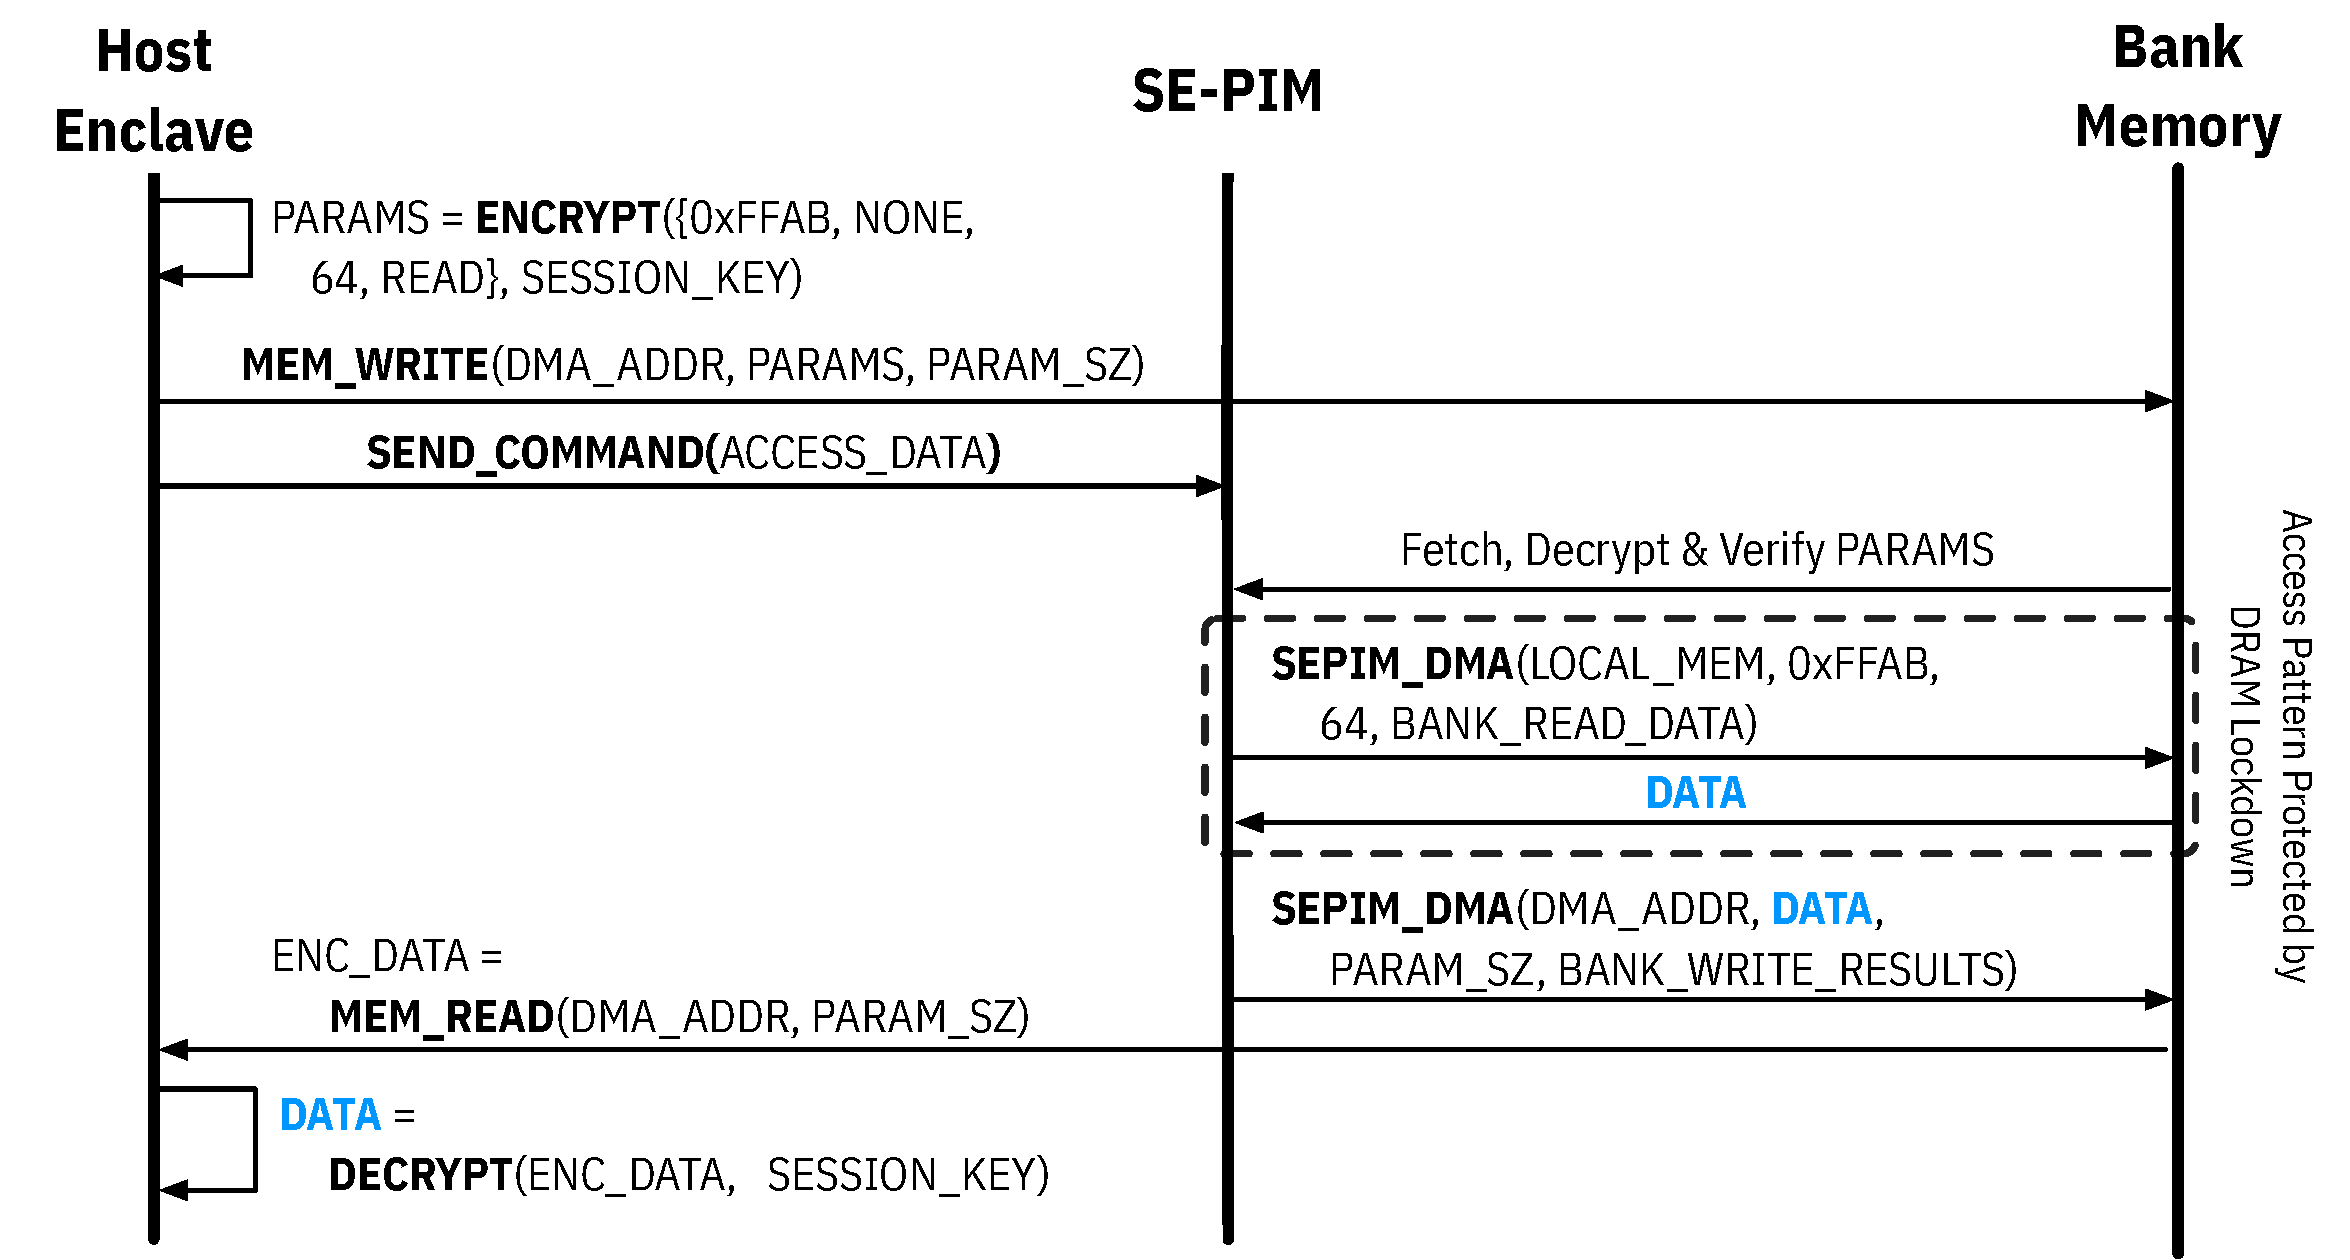
\includegraphics[width=0.90\columnwidth ]{figures/sepim/secure_access.pdf}
    \caption{An example of data read using controlled memory access channel. The data access pattern of host is protected by encryption, while the data access pattern of PIM kernel is protected by DRAM lockdown.}
    \label{fig:secure-access}
\end{figure}

\hdr{Controlled data access.} \texttt{ACCESS\_DATA} allows the host enclave to read or write a block of data during bank lockdown while hiding the access pattern from observers. Parameters for \texttt{ACCESS\_DATA} are the encrypted data block, the requested address, the size of access, and the type of operation (read or write). Instead of introducing separated commands for data read and write, we define the type of access in the parameters to mimic the security guarantees of oblivious RAM algorithms~\cite{path-oram}. \autoref{fig:secure-access} shows the data access from the host enclave using \texttt{ACCESS\_DATA}. First, the encrypted parameters are written into the DMA-based secure channel, and the command is sent to the \thename unit. The \thename unit will decrypt and fetch the memory request into its local memory on receiving the commands. The data block is placed in the requested location for a write request. Otherwise, on reading requests, the \thename unit fetches the block, encrypts, and writes it to the secure channel. Collaboration from the host enclave is required to achieve full ORAM-like security properties. Namely, to hide the type of memory access, the memory requests must contain dummy data on a read, and a dummy read request must follow every write request.

\hdr{Controlled data movement.} The \texttt{MEMCPY} command instructs \thename to copy data from one address to another, which is useful when data is already located inside the memory. On receiving the command, \thename will fetch the requested data block to local memory and write it to the destination address. The operation performs data movement using the fast internal bus on PIM, which reduces expensive data transfers on the memory bus.

% \hdr{Controlled data movement.} 







\section{SE-PIM Programming Model}
\label{sec:prog-model}
%\hjc{What does this achieve??? This is like a instruction manual for PIM programming. No explanation on its purpose, advantages, and our contribution. Unnecessary long and pointless. REWRITE}

In this section, we explain the programming model of \thename. Our proposed framework presents an abstraction on top of the \thename architecture we introduced. Our programming model supports the two design objectives of \thename that we outline in \cref{subsec:objectives}: a secure memory extension and a secure large data accelerator for the secure enclave. We elaborate the software components of \thename that help an enclave interact with \thename in \cref{subsec:software}. Then, we go through the design of our programming model that enable our design objectives in \cref{subsec:prog-model}.

%We first describe the interfaces between the host enclave and \thename in \cref{subsec:interfaces}. Then, we illustrate the programming model of offloading computations to \thename and using \thename as secure memory extension through code examples (\cref{subsec:prog-model}).



\subsection{Software Components}
\label{subsec:software}
%The software components of \thename includes the facilitates the usage of \thename from a secure enclave. 
As the programming model of SGX enclaves does not support a trusted I/O path, the communication channel between the enclave and the devices has to be set up by the untrusted kernel and host application. Hence, there are untrusted and trusted components in our software infrastructure. Our trusted software includes the enclave host program, the trusted \thename user library, and the \thename kernel. Our untrusted components are the kernel driver and the untrusted user library. The untrusted components only set up the secure communication channel; after a secure session is established, all communication between the enclave and \thename is encrypted and authenticated.
%\subsection{Overview}
%\hdr{\thename host application.}

\hdr{\thename driver and user library.}
The communication interfaces between the host and the \thename unit are initialized by the driver and the user library. The driver maps the physical addresses corresponding to the memory banks in the \thename-enabled memory modules into the host kernel address space. It also maps the registers of each \thename unit to expose the device control channel to the host. In order to provide access to \thename, the driver creates a virtual file interface to the host library in the user space (e.g., \texttt{/dev/pim0}). A user library at the host side is required to allow an in-host program to communicate and send workloads to \thename. The \thename library has two components, a trusted part that resides in the enclave code and an untrusted part in the host program. The untrusted part of the library initializes the communication interfaces by obtaining the device driver's memory banks and control registers. The trusted library contains functions that facilitate the communication between the enclave and \thename units (e.g., transfer data to the memory bank and sending commands to \thename).



%The driver and the user library help the host enclave establish communication channels with the \thename units.  
\hdr{Enclave host program and \thename kernel.}
The enclave host program contains the confidential computation logic that uses \thename as its accelerator. \thename kernel includes protected functions to be executed inside \thename. The developer of the host enclave must select the computation (e.g., functions) to be offloaded, then implement and cross-compile them for \thename platform. 
% The kernel objects are linked with a runtime library with helper functions for PIM operations (e.g., sending DMA requests to the memory bank). 

The similar to the interfaces of \baseline, host enclave communicates with the \thename kernel running on the \thename unit core through two physical interfaces (described in \cref{subsec:pim-baseline}): \emph{memory-mapped registers} and \emph{direct memory access (DMA)}. On the two interfaces, we establish two communication \emph{channels}. The \emph{command channel} (CMD CH) use the memory-mapped registers to issue \emph{commands} (listed in \autoref{tab:commands}) to the PIM core to control its execution.  

The \emph{parameters channel} (PARAM CH in \autoref{fig:interfaces}) uses DMA to send parameters of the commands. It functions as a secure communication channel between the host enclave and a \thename unit. Messages through the channel are encrypted using a shared session key (\texttt{SESSION\_KEY}) yielded during the initial attestation and key exchange~(\cref{subsec:attestation}). On \texttt{EXECUTE} commands, the parameters become the arguments for execution that is defined by the \thename kernel.


%It uses the memory mappings obtained by the untrusted driver and user library to send commands and parameters to \thename.

%A common header file is also employed for shared data structures (e.g., \texttt{SE\_PIM\_params\_t}) between \thename kernels and the host process.

%\subsection{Using \thename as a Secure Memory Extension}
% \hjc{Too many subsections A through L is too many.}







%Before the execution of a \thename kernel, the host sends parameters containing the function name (FN) to be executed and the arguments (FN ARGS) to the \emph{parameter channel} (PARAM CH). 


% We also demonstrate an overview of our execution model in \autoref{fig:interfaces}. 
% 
% \hj{The previous claim was that zero-copy is possible?}

%\hj{You said the regions are accessed just like normal memory. But we use DMA?}

% \todo{Mention Zero-copy...}


% \hjc{This requires explanation of RA components in the hardware}



% \hjc{Maybe merge secure comm ch. with remote attestation?}

% \hdr{The encrypted parameter channel.}
% \hdr{Secure communication channel.} 
%The host enclave communicates with the PIM kernel running on the \thename unit core through two physical interfaces: \emph{memory-mapped registers} and \emph{direct memory access (DMA)}. % For DMA, the host process maps the buffer into its own memory space. 
% On the two interfaces, we establish two communication \emph{channels}. The \emph{command channel} use the memory-mapped registers to issue \emph{commands} (listed in \autoref{tab:commands}) to the \thename core to control its execution. For each \thename core, there is a corresponding control register. For instance, writing an \texttt{EXECUTE} command to a control register tells a \thename core to start executing the kernel. 


%\hdr{Data loading through the data channel.}  Therefore, we allow directly writing of data into the memory bank before starting PIM computation for efficient data transfer between host and PIM. After the initial transfer finishes, the memory bank can enter a \emph{lockdown} mode to protect data confidentiality and integrity (\cref{subsec:access-control}).


%\subsection{Extending Enclave Memory with \thename}

\subsection{SE-PIM Usage Model} 
\label{subsec:prog-model}
\label{subsec:accelerator-model}

% SE_PIM_cert_t *cert = se_pim.get_cert(); |\label{line:attest_start}|
% remote_attest_and_exchange_keys(se_pim, cert);
% se_pim.offload_kernel("kernel.elf.enc"); |\label{line:attest_end}|
%transfer_data_to_mem(ptr_A, ptr_B);
% // Use the secure interface to access data from memory
% se_pim.read(data_read, ptr_A, DATA_SZ);
% se_pim.memcpy(ptr_A, ptr_B, DATA_SZ);
% void *ptr_B = se_pim.transfer(data_B, size_B);



% \begin{figure}[t]
    \begin{listing}[h]
    \centering
\begin{minted}[linenos=true,escapeinside=!!]{c}
// Initialize and and attest a SE-PIM unit
SE_PIM *se_pim = SE_PIM_init(MEM_MODULE_ID,
                                       BANK_ID, 
                                       "kernel.elf.enc"); !\label{line:object}!
// Transfer the data to SE-PIM memory bank
void *ptr = se_pim.transfer(obj, DATA_SZ); !\label{line:transfer_start}!

se_pim.lock_mem(); !\label{line:transfer_end}!

// Send command, execute and get result
SE_PIM_params_t params = {.fn = "increment", 
                                   .data_ptr = ptr, 
                                   .size = DATA_SZ};

for (int i = 0; i < ITERATIONS; i++)
    SE_PIM_result_t *result = se_pim.execute(params);

se_pim.read(result, ptr, DATA_SZ); !\label{line:secure_access}!
\end{minted}
    \caption{Host-side code snippet illustrating computation offloading to \thename.},
    \label{lst:accelerator},
\end{listing}

% \end{figure}

\autoref{lst:accelerator} demonstrates the code example of a host-side enclave that uses a \thename unit as an accelerator. The enclave first obtains an object representing a \thename unit with the library function call \texttt{SE\_PIMInit} (line \ref{line:object}). It performs remote attestation and key exchange during initialization, then offloads the encrypted \thename kernel to the \thename unit. Then, it transfers encrypted data object into the memory banks through the direct mapping and instructs the \thename unit to \emph{lock} the memory bank (lines \ref{line:transfer_start}-\ref{line:transfer_end}). The enclave then generates a parameter structure (\texttt{SE\_PIM\_params\_t}) consisting of the in-kernel function name, the pointer to the data to be processed, and the size. It then commands the \thename unit to start execution in multiple iterations while keeping the data protected inside the memory. Finally, the host read the result from the memory bank (line \ref{line:secure_access}).


%\hdr{Zero-copy}
\hdr{Extending enclave memory with \thename.} 
To support our objective as a secure memory extension for processor enclaves, our user library provides functions to offload data into the protection of \thename and access data without leaking data access patterns on the memory bus. Our data loading function (line \ref{line:transfer_start} of \autoref{lst:accelerator}) uses direct memory mappings to efficiently load data into the \thename memory banks without compromising security. As we discussed in \cref{subsec:access-control}, the act of sequential data loading does not generate distinguishable access patterns. Furthermore, we observe in \cref{subsec:secure-access-eval} that there are overheads when using the controlled memory access channel that is side-channel resistant, which would inevitably create overheads for large data transfers. After the initial transfer, the enclave commands the memory bank to enter \emph{lockdown} to protect the data inside memory (explained in \cref{subsec:access-control}).

After DRAM lockdown, data within memory is accessed through the user library functions \texttt{read()}, \texttt{write()} and \texttt{memcpy()}. The functions internally create encrypted memory requests to the controlled memory access channel (demonstrated in \cref{subsec:secure-access}), and let \thename perform the actual data access. Hence, the data access pattern is protected from any observing attacker. In the example in \autoref{lst:accelerator}, the host enclave use the function \texttt{read()} to read the incremented data block from memory without leaking the requested address and the type of operation (line \ref{line:secure_access}).

\begin{figure}[h]
    \centering
    \begin{minted}[mathescape,escapeinside=||]{c}
void increment(data_ptr, size){
    char local_mem[BATCH_SZ];
    SE_PIM_result_t result;
    result.count = 0;
    // Request data from bank memory 
    for (int i = 0; i < size / BATCH_SZ; i++){
        sepim_dma(data_ptr + BATCH_SZ * i, local_mem, |\label{line:dma_read}|
                      BATCH_SZ, BANK_READ_DATA);
        // Process data in local memory
        for(int j = 0; j < BATCH_SZ; j++){ |\label{line:process_start}|
            local_mem[i] += 1; 
            result.count++;} |\label{line:process_end}|
        sepim_dma(local_mem, data_ptr + BATCH_SZ * i, |\label{line:dma_write}|
                     BATCH_SZ, BANK_WRITE_DATA);
    }
    return_result(&result);|\label{line:return}|
}
\end{minted}
    \caption{\thename kernel code snippet showing the kernel fetches data into local memory, increments, writes updated data to bank memory, and finally returns the results to the enclave.}
    \label{lst:kernel}
\end{figure}

\hdr{Offloading confidential computation to \thename.}
\autoref{lst:kernel} demonstrates the kernel logic used in \autoref{lst:accelerator}. 
After remote attestation and key exchange, the encrypted \thename kernel binary is offloaded through the secure channel as the argument to the command \texttt{LOAD\_KERNEL}. The kernel is loaded into \thename local memory and used by the PIM core for execution. Then, the PIM core takes the measurement (i.e., the hash) of PIM local memory and sends the measurement to the host enclave. The host enclave can use this measurement to verify the software state of a \thename unit. After loading the PIM kernel, the \thename unit goes into an idle state and waits for future commands (e.g., \texttt{EXECUTE} or \texttt{LOCK\_MEM}). 

\thename makes use of the \emph{zero-copy} model of PIM-based computation, as described in \cref{subsec:pim-baseline}. Data is not moved for computation, but only the \emph{pointers} to the data are embedded in function arguments. \thename uses the pointers to fetch the actual data from the bank memory into its local memory and perform the requested operation on the data. This eliminates the data transfers for each computation and makes use of the fast internal bus of PIM systems~\cite{hmc,primer-on-pim}. Moreover, the computation does not leave any pattern on the memory bus. This is only possible on PIM-based computation since CPUs, or any accelerators on the peripheral bus, inevitably access memory with patterns unless using ORAM primitives. To command a \thename unit to execute the kernel, the host sends the encrypted parameters through the encrypted parameter channel; then sends an \texttt{EXECUTE} command to the corresponding \thename unit. After execution, \thename kernel encrypts and returns the execution results to the enclave through the same encrypted channel (\ref{line:return}).

%There are two types of computational results from PIM. 
%First, the \thename kernel might update the data inside the memory due to the computation. For instance, the kernel in ~\autoref{lst:kernel} increments the values in an in-memory array by one. The host retrieves the data with the controlled memory channel proposed in \cref{subsec:secure-access} to hide the address side-channels. Second, the computation results can be information obtained from the data inside the memory content. This type of result is similar to the return value of functions calls. For instance, in \autoref{lst:kernel}, the kernel calculates a statistic (the count of elements) that is obtained based on the data. The result is encrypted with the session key and written to the secure communication channel. 
%\hdr{Loading \thename kernels.} 

%The kernel fetches data from the memory bank to its local memory, increments it, and then writes it back to the same location. Data is processed in batches, for each batch, the kernel initiates DMA transfers through built-in functions \texttt{dma\_request()} to load and decrypt data from the memory bank into \thename local memory (line \autoref{line:dma-read}). It then processes data in the local memory (lines \autoref{line:process-start}-\autoref{line:process-end}). Finally, the kernel updates the memory bank's content with a DMA transfer in the opposite direction (line \autoref{line:dma-write}).
%The kernel also keeps track of the number of elements it accessed. It returns the count of elements as the computation results through the secure channel (line \autoref{line:return}).



%\hj{leave only absolutely necessary code}



% the index of the targeted memory bank (housing a \thename unit) and memory module 

%The programming model of \thename also adapted by many previous works~\cite{upmem,tesseract,impica,neural-network-training}. 







%\hdr{Initialization and \thename kernel loading.} 
%The untrusted host library first obtains the memory mapping of the memory bank and the control registers from the driver with a memory mapping request (\texttt{mmap()}) on the virtual file interface of the driver. Then, the trusted runtime library initializes an object (line \autoref{line:object} in \autoref{lst:accelerator}) that contains a \thename unit mappings, the memory allocation status, and functions that help the enclave communicate with \thename units. When multiple \thename units are employed, a \thename object is created for each \thename unit. 
%\hdr{\thename attestation and keys exchange.}
%The host enclave then uses the communication interfaces (i.e., the virtual mapping) to send attestation requests to \thename units. After, the host enclave exchanges a session key and a data decryption key with the \thename unit. \thename and the host enclave use the session key to encrypt all messages on the secure communication channel from this point onward. We describe the attestation and key exchange processes in more detail in \cref{subsec:attestation}.  %Since \thename units use the same root endorsement key

%\hdr{Transfering encrypted data to \thename memory banks.} Different from the programming model of GPUs that requires a DMA buffer to transfer data from and to the VRAM~\cite{graviton}, the host use uncached memory mapping to transfer encrypted data directly to the \thename memory banks. After data transfer finished, the host enclave commands \thename to enable DRAM lockdown (\cref{subsec:access-control}).  %The data transfer only occurs before the execution of the \thename kernel; after, the access to the memory bank is \emph{locked}, except for accesses to the DMA-based communication channel.

%\hdr{Execution of \thename kernels.}  %Securing the execution of the kernels are discussed in \cref{sec:secure-acc}. 
%Note that no additional data transfer is needed for the execution of the kernel. The host only sends the \emph{pointer} of data to be processed inside memory, which the kernel will use to fetch the data by itself with DMA transfers. 


%\hdr{Execution of \thename kernel and results retrieval.} 







% Note that all of the commands on \thename share the same parameter passing method described in the next section. However, the
% and key storage that only allows indirect interactions with the root endorsement key (\texttt{EK}) through a predefined set of commands.


\section{Implementation}
\label{sec:implementation}
We implemented a prototype of the \thename design using a cycle-accurate full system simulation~\cite{gem5}. Regarding the low-level simulation configurations,  we referenced well-documented industry-grade products~\cite{upmem} and simulation configurations from other works on PIM ~\cite{smcsim,obfusmem,ambit,tesseract}. Our simulation is well modularized and generalizable; the hardware components that we implement can be easily modified and provides well-defined APIs for writing host-side and PIM-side applications. 

%In our simulation, the PIM cores are modeled as general-purpose processing cores.

\begin{figure}[h]
    \centering
    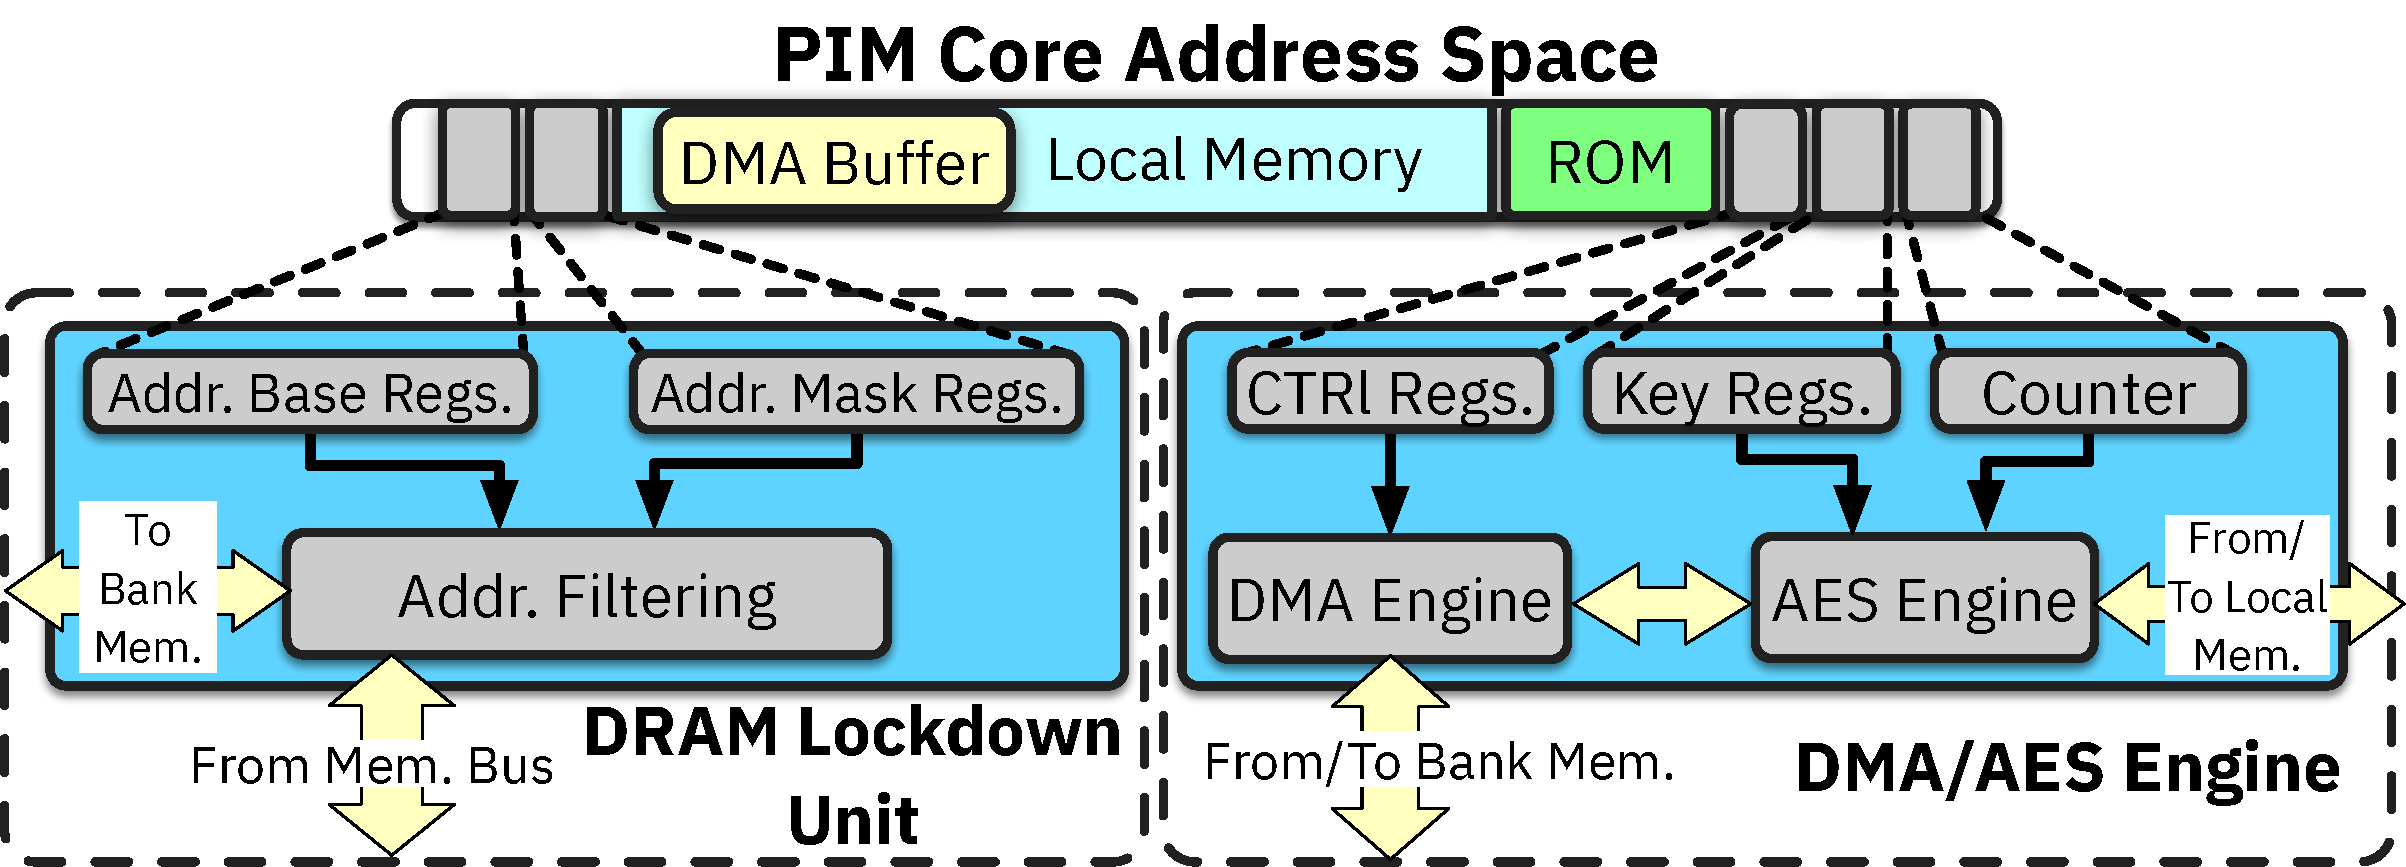
\includegraphics[width=.8\textwidth]{figures/sepim/implementation.pdf}
    \caption{The address space of a PIM core. The control registers of the DRAM lockdown unit and the AES-enabled DMA engine is mapped into the address space of the PIM core for MMIO communication.}
    \label{fig:access-control-dram}
\end{figure}

% \hdr{Simulating PIM systems. } Each PIM core is implemented as a separated simulation system.

% gem5 allows for multiple systems to be simulated simultaneously. This allows us to implement each PIM system as a separated system, and connect them to the host using

% The DMA channel is configured upon device initialization by the host enclave writing the address and size of the DMA region into the registers of the PIM core. The configuration step is necessary because since we disallow the host to access PIM local memory directly (\cref{subsec:memory}), there is no other method to set up the DMA channel for parameters of commands. The content passed through this channel is encrypted with the session key shared after the key exchange using AES-GCM with a counter to prevent replay attacks. The PIM core retrieves the parameters the same way it fetches encrypted batch of data into local memory, using the AES-enabled DMA engine (\cref{subsec:performance}). The exact mechanism for parameter transfer is also applied.

% \subsection{Read-only Memory}
% We implement the Read-only memory, which contains several methods for key exchange and attestation inside 

%\subsection{\thename Core Address Space}


\begin{table*}[t]
    \centering
    \begin{threeparttable}
    \footnotesize
	\renewcommand{\arraystretch}{0.9}
	\renewcommand{\theadgape}{\Gape[.2pt]}
  	\renewcommand\theadfont{\bfseries}
    \begin{tabular}{p{2.5cm}p{3.2cm}p{3.5cm}p{4cm}}
        \toprule
        \thead{Command}&\thead{Parameters}&\thead{Results}&\thead{Description}\\
        \midrule
        \texttt{GET\_CERT\textsuperscript{\dag}}              & - & \texttt{PIM\_CERT} &         Get \thename's certificate\\ 
        \texttt{SET\_SESSION\_KEY}      & \texttt{SESSION\_KEY} & - & Send encrypted session key to PIM\\ 
        \texttt{SET\_DATA\_KEY}         & \texttt{DATA\_KEY} & - & Send data decryption key to PIM\\ 
        \texttt{LOAD\_KERNEL}           & \texttt{KERNEL\_BINARIES} & \texttt{LOCAL\_MEM\_MEASUREMENT}&         Load PIM kernel\\
        \texttt{EXECUTE}\textsuperscript{*}                & \texttt{FN\_NAME, FN\_ARGS} & \texttt{RESULTS} &         Command PIM to execute the kernel\\ 
        \texttt{LOCK\_MEM}              & - & \texttt{BANK\_MEASUREMENT} &         Enable DRAM lockdown\\
        \texttt{MEMCPY}                 & \texttt{DST\_ADDR, SRC\_ADDR, SZ} & - &         Move data within the memory bank during lockdown mode\\        
        \texttt{ACCESS\_DATA}           &\texttt{DATA, ADDR, SZ, OP}& \texttt{DATA} &         Data access during lockdown mode\\        
        \texttt{UNLOCK\_MEM}            & - & - & Disable DRAM lockdown\\
        
        \texttt{DESTROY}\textsuperscript{\dag}                & - & - &         Stop \thename execution, clear local memory and unlock bank\\
        \bottomrule
    \end{tabular}
    
	\begin{tablenotes}
	    \item \hfil \textsuperscript{*} parameters and results are defined by \thename kernel; \textsuperscript{\dag} does not require authentication.
	  %  \textsuperscript{*} data is contained on user's device;
% 			\item \hfil\textsuperscript{\dag};
% 			\textsuperscript{*}
		\end{tablenotes}    
    \end{threeparttable}
    
    \caption{Commands supported by \thename, their parameters, results, and descriptions.}
    \label{tab:commands}
\end{table*}


\subsection{PIM Core and ROM}
We implement the PIM cores as general-purpose execution cores that use the local memory as their RAM and have low-latency access to the memory banks. The specifications for the cores are described in~\autoref{table:config}. \autoref{fig:access-control-dram} demonstrates the address space of the PIM core and the memory mapping of the components into the address space. Local memory is mapped into the address space of \thename as a contiguous memory region, which it uses as the memory for its code (the \thename kernel), the stack space, and DMA transfers. The PIM core communicates with other hardware components using MMIO. The registers of the AES-enabled DMA engine and the DRAM lockdown unit are memory-mapped to fixed addresses so that the PIM core can configure and send commands to the components.

ROM contains the code for cryptographic primitives (e.g., key generation) and functions for handling the commands. The list of supported commands is demonstrated in \autoref{tab:commands}. Our prototype implements ROM code directly inside the PIM kernel code and loads it to the local memory. This would simplify the implementation while achieving the same functionality and performance characteristics. ROM must be implemented in a separated read-only memory module to protect the security-sensitive code against tampering in an actual implementation. Moreover, PIM core should be implemented so that only the attestation code can access the key storage containing the root endorsement key to prevent key leakage. As noted by \cite{minimalist}, the requirement can be easily enforced with an introduction of a hardware monitor on a PIM core's program counter that only allows access to the EK when the PC is within the attestation code.

%Finally, it is crucial to prevent a malicious enclave from leaking the EK. First, we only allow the attestation procedure to access the EK.  Moreover, for each newly created \pimenclave, a new public and private key pair used for attestation is derived from the EK to prevent information leakage. 
% \subsection{ROM}

\subsection{AES-capable DMA Engine}
\label{subsec:impl-aes}
We implemented and incorporated the AES-GCM acceleration capability in the DMA engine of the PIM core package. Our strategy in incorporating a hardware design into the simulation was two-track: we first modified the DMA engines in the memory controller of the PIM core package to include AES-GCM acceleration hardware to test the correctness aspect. Then, we calculated the increased number of cycles consumed for each DMA transfer by inspecting the specifications of AES hardware specifications.


\begin{figure}[t]
    \centering
    \caption{The definition of \texttt{sepim\_dma} inside a \thename kernel. The function uses the control registers of the DMA/AES engine mapped into PIM's address space.}
    \label{lst:aes}
\begin{minted}{c}
void sepim_dma(src, dst, sz, cmd){
    write_reg(DMA_SRC_ADDR_REG, src); 
    write_reg(DMA_DST_ADDR_REG, dst); 
    write_reg(DMA_SZ_REG, sz); 
    write_reg(DMA_CMD_REG, cmd);
    // Wait for transfer to finish
    wait(DMA_STATUS_REG);
}
\end{minted}
\end{figure}


% \vspace{5pt}

\hdr{Functional correctness.} We implemented AES functionality in the memory controller and its DMA engine of each PIM core. The implementation is based on open hardware IPs~\cite{aes-opencore,nxp} and uses functions from the \texttt{OpenSSL} library. We expose the configuration registers for various configuration parameters and commands by mapping them into the PIM core address space (\autoref{fig:access-control-dram}). Through the commands, the PIM core can specify whether the direction of data indicates whether decryption or encryption should be performed; decryption is used to transfer from the memory bank into PIM local memory bank and vice versa. The DMA engine also uses different encryption keys (\texttt{SESSION\_KEY or DATA\_KEY}), depending on the command. Upon receiving a command from the PIM core, the DMA engine initiates the transfer, then encrypts or decrypts the contents appropriately. \autoref{lst:aes} demonstrates the function \texttt{sepim\_dma()} that use  the AES-capable DMA engine for encrypted data movement.


% \begin{scriptsize}

% \end{scriptsize}

% \hdr{Encrypted data format and size.} Data is partitioned into encrypted blocks, each of which has an encryption IV and a tag appended to them for decryption. In particular, the size of each block should be

% \vspace{2pt}
% \begin{equation*}
% \footnotesize
% size_{block} = \frac{size_{available} - n_{split} * (size_{IV} + size_{tag})}{n_{split}},
% \end{equation*}
% \vspace{2pt}

% where $n_{split}$ is the number of encrypted data blocks that fit into the local memory in one transfer. The developer can customize this value to optimize fetching and processing in \thename kernel. $size_{IV}$ and $size_{tag}$ are the sizes of IV and tag used in decryption and authentication, and $size_{available}$ is the maximum available size used to contain the data inside PIM local memory. Finally, the total number of encrypted blocks with respect to the data size is

% \begin{equation*}
% \footnotesize
% n_{blocks} = \frac{size_{data}}{size_{block}}.
% \end{equation*}
% \vspace{1pt}

\hdr{Simulating latency. } The performance overhead of incorporating AES-GCM acceleration into DMA engines is well-studied and can be accurately estimated. We adapt the latency described in the specification of the IP~\cite{aes-opencore}. Also, previous works have estimated the latency of almost identical hardware~\cite{invisimem, obfusmem}. We estimated that the AES-GCM accelerator can operate at a $300$MHz clock rate and could encrypt 128-bit blocks each cycle. Based on the estimation, we add a delay of $1$ cycle to each 16 bytes data chunk processed by the DMA engine in our simulation.



% After keys exchange with the host enclave is finished, the PIM core then configures the AES engine with the shared key inside the AES engine and reset the counter register. The counter value increments monotonically at each encryption and decryption, which is utilized to protect the messages against replay packets by binding them with the plain text value. 




% Inside of the simulation, the request to the AES engine is handled by the \texttt{recvAtomic} function inside of PIM's memory controller. It reads the content of the packet to get the command, then performs functional decryption of the content of \texttt{PIM\_AES\_INPUT}. Finally, the result is written into \texttt{PIM\_AES\_OUTPUT} so that the program can collect it.




% {
% \footnotesize
% \begin{code}{C}
% Tick PIMLocalMemory::recvAtomic(PacketPtr pkt) 
% {
%   ...
%   if (pkt->getAddr() == PIM_AES_CMD_ADDR) {
%     switch (get_content(pkt)): 
%       case AES_DECRYPT_MESSAGE:
%         functional_decrypt(PIM_AES_INPUT_ADDR, 
%                           PIM_AES_OUTPUT_ADDR,
%                          PIM_AES_COUNTER_ADDR,
%                             PIM_AES_TAG_ADDR);
%         write_memory(PIM_AES_STATUS_ADDR, 
%                                AES_DONE);
%     break;
%   case AES_ENCRYPT_MESSAGE:
%     ...
%   }
%   ...
% }
% \end{code}
% }



\subsection{SE-PIM DRAM Lockdown Unit} 
% \hdr{Access control in DIMM-based memory.}
% \autoref{fig:access-control-dram} shows our proposed design of the access control logic for DDR4 at the memory bank level. In the DRAM module, each incoming bus address is translated into a combination of \emph{bank group}, \emph{bank address}, \emph{row address} and \emph{column address}. Access control using the requested address can be enabled by introducing range checks for column and row addresses. In our design, the range-checking logic implements a pair of \emph{range mask} and \emph{range base} registers that are exposed to the PIM core for configuration. 
% \new{
% Circuits that consist of AND and XNOR gates are added that take the column/row address of memory accesses as the input. The circuit will only generate a "true" output when a column/row address falls within the preconfigured address range (i.e., between range base and range base plus range mask). 
% A \emph{data gate} is introduced to collect the checks from the introduced circuits and only allow data access when both checks permit the access.
%The memory accesses are only allowed if both checks for column and row addresses succeed.
% }
% Our access control unit is similar to the circuit structure that already exists in processors to detect illegal memory accesses~\cite{sgx-explained}. Finally, setting the range base and mask registers to \texttt{0x0} will disable the access control. We expect that the proposed access control logic can be incorporated into DDR4 DRAM modules and 3D-stacked memory modules. We estimate that our range check logic, comprised of simple logic gates~(e.g., $10$ AND and $9$ XNOR gates to check 10-bit addresses), will introduce a negligible latency. For instance, in a typical DDR4-3200 module, row activation and column accesses take approximately $15ns$ and $24$ cycles, respectively~\cite{micronddr4}. The latency of row and column accesses can easily mask the latency of our access control logic.

We discuss the implementation of the DRAM lockdown unit in different PIM architectures. For 3D-stacked memory, the implementations often use packetized interfaces that replace the traditional low-level DDR commands~\cite{hmc-spec,invisimem,hmc}. Hence, inserting the logic for denying access to a region inside memory is straightforward. Many works have taken advantage of the flexibility of 3D-stacked memory to incorporate authenticated encryption into the packet handling logic ~\cite{invisimem,obfusmem}. Therefore, we expect our proposed logic change that implements DRAM lockdown can be easily incorporated into 3D-stacked PIM hardware. On the other hand, it is more challenging to implement a filtering mechanism on DIMM-based memory since the DDR interface is very sensitive to timing differences~\cite{micronddr4}. Hence, we focus on the 3D-stacked memory-based implementation in this work.


% \hdr{Access control in DIMM-based memory.}
% It is more challenging to implement an access control mechanism in DIMM-based memory, as the DDR interface is very sensitive to the timing difference.
%In DIMM-based memory, the access control unit is similar to the circuit structure that already exists in processors to detect illegal memory accesses~\cite{sgx-explained}. Finally, setting the range base and mask registers to \texttt{0x0} will disable the access control. We expect that the proposed access control logic can be incorporated into DDR4 DRAM modules and 3D-stacked memory modules. We estimate that our range check logic, comprised of simple logic gates~(e.g., $10$ AND and $9$ XNOR gates to check 10-bit addresses), will introduce a negligible latency. For instance, in a typical DDR4-3200 module, row activation and column accesses take approximately $15ns$ and $24$ cycles, respectively~\cite{micronddr4}. The latency of row and column accesses can easily mask the latency of our access control logic.

\hdr{Simulating DRAM lockdown.}
To simulate DRAM lockdown, we introduce an \emph{address filtering mechanism} into the packet handling logic of the memory. We mapped two registers, \emph{address start} and \emph{address mask} to the address space of a PIM core, which it can use to configure the protected address range (\autoref{fig:access-control-dram}). The address start register specifies the start of the protected address range. The address mask register is combined with the address start register to specify the upper bound of protected addresses. In our simulation, we made modifications to the \path{AbstractMemory} object in gem5, which is an abstraction of the memory-side memory controller. As \path{AbstractMemory} uses packets to interact with other components, its functionality is similar to how the logic layer of 3D-stacked memories handles the requests.
It is rather challenging to accurately simulate the latency of such a low-level mechanism in a simulator or even FPGAs. We leave actual hardware implementation and verification of the DRAM lockdown unit as future work. 

% We inserted a check to every packet received by the memory controller to serve an empty packet if the request falls into the protected address range indicated by the two registers.




\begin{table}[t]
    \scriptsize
	\renewcommand{\arraystretch}{0.5}
	\renewcommand{\theadgape}{\Gape[.2pt]}
% 
%   	\renewcommand\theadfont{\bfseries}

 	\centering
    \begin{subtable}{\columnwidth}
    
 	    \centering
% 	\begin{adjustbox}{width=.9\columnwidth}
		\begin{tabular}{p{20mm}p{55mm}}
    		\toprule
			\multicolumn{2}{c}{\thead{Host Configuration}}\\ 
            \midrule
			\thead{Processor} &  \makecell[l]{8 in-order ARMv7 cores \\ (2 threads/core, clock rate $4.0$ GHz)}\\
			\midrule
			\thead{L1 Cache}  & Per-core, $32$ KB I-cache, $64$ KB D-cache \\
			\midrule
			\thead{L2 Cache}  & Shared across cores, $256$ KB\\  
% 			\hline
            \midrule
			\thead{OS} & Linux kernel 3.16.0-rc6 \\
			
			\bottomrule
% 			% \renewcommand{\arraystretch}{0.1}
% 			% \multicolumn{2}{c}{}\\«
		\end{tabular}
	\end{subtable}
% 	\end{adjustbox}
 	\rule{0pt}{1ex}
%  	\vspace{1mm}
% 	\newline
% 	\begin{adjustbox}{width=.9\columnwidth}
    \begin{subtable}{\columnwidth}
 	\centering
		\begin{tabular}{p{20mm}p{55mm}}
		    \toprule
			\multicolumn{2}{c}{\thead{PIM-enabled Memory Configuration}}\\
		    \midrule	
			\thead{Memory Banks} & \makecell[l]{8 PIM-enabled memory banks, $64$ MB/bank, \\Memory type: \texttt{gem5} \texttt{HMCVault}}  \\
			\midrule
			\thead{PIM Core}  & \makecell[l]{1 $\times$ in-order ARMv7 core per bank \\(1 thread/core, clock rate $1$ GHz) }                           \\
			\midrule
			\thead{Local memory} & $1$ MB per core\\
			\bottomrule
		\end{tabular}
		
    \end{subtable}
% 	\end{adjustbox}
% 	\vspace{1mm}
% 	\newline \begin{adjustbox}{width=1\columnwidth}
% 		\begin{tabular}{p{20mm}p{60mm}}
% 			\toprule
% 			\multicolumn{2}{c}{\bfseries DRAM Configuration}                        \\
%             \midrule
% 			\bfseries DRAM parameters & Row buffer size: 256B, burst size: 32B
% 			tRP: 13.75ns, tRCD: 13.75ns, tCL: 13.75ns, tBURST: 3.2ns                    \\
%         	\bottomrule
% 		\end{tabular}
% 	\end{adjustbox}
	\caption{Configuration of the simulated system.}
	\label{table:config}
\end{table} 

\begin{figure*}[t]
  \centering
  \begin{subfigure}{.8\textwidth}
  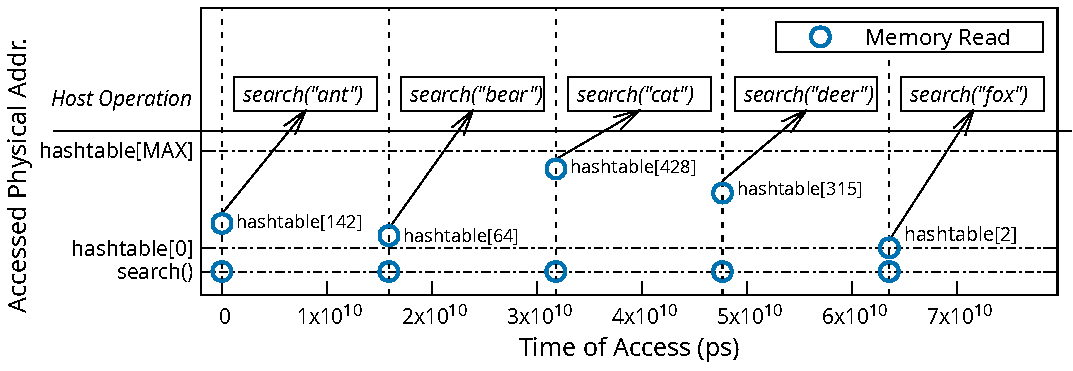
\includegraphics[width=.975\columnwidth]{figures/sepim/host-access-pattern.pdf}
  \caption{Memory access pattern observed on memory bus during host enclave dictionary lookup.}
  \label{fig:host-pattern}
  \end{subfigure}
\begin{subfigure}{.8\textwidth}
  \centering
  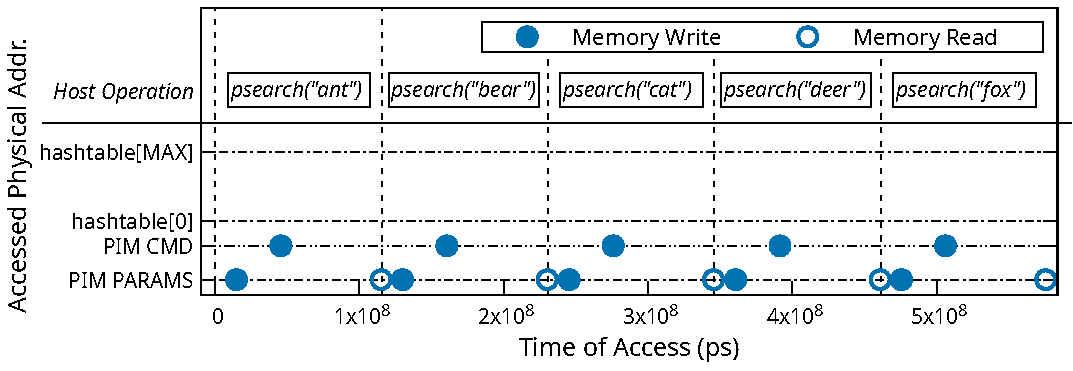
\includegraphics[width=.975\columnwidth]{figures/sepim/pim-access-pattern.pdf}
  \caption{Memory access pattern observed on the memory bus during \thename-assisted dictionary lookup.}
  \label{fig:pim-pattern}
  \end{subfigure}
  \caption{Memory access pattern observed on bus during confidential \texttt{hunspell} dictionary program. In host CPU enclave-only model, accessed \texttt{hashtable} location reveals  looked up word. In \thename-assisted model, observed memory pattern is consistent for all looked up words.}
  \label{fig:access-pattern}
\end{figure*}

\section{Evaluation}


%\fix{Do we evaluate robustness against side-channels?}
We evaluated \thename through a cycle-accurate simulation. The simulation configuration we used for simulating our system can be found in \autoref{table:config}. Note that we assume the presence of processor enclaves in the host, as our simulator does not support simulation of enclaves such as SGX~\cite{sgx} or TrustZone~\cite{arm-tz}. We assume that \thename cooperates with the host enclave to achieve confidential computation. For this reason, we did not consider the overhead from the use of host processor enclaves, although the exclusion of the overhead works against our favor. We configured the PIM core to operate at the clock rate of $1$ GHz to reflect the power and area constraint in the DRAM or 3D-stacked memory packages. The timing parameters used for the simulation were determined through existing works that conducted simulations on similar hardware~\cite{smcsim,concurrent-data,tesseract}. There are 8 \thename-enabled memory banks inside the memory module that can execute independently. We take advantage of all 8 \thename-enabled memory banks in the data-intensive performance evaluation in \cref{subsec:app-perf}. Other benchmarks use only a single memory bank.

Our evaluations show vital aspects of our design: first, we show that offloading computations to \thename leak no address-based side-channels on the bus. Second, we show that our introduced modifications do not inhibit PIM's ability to perform data-intensive computation efficiently. Finally, we also demonstrate \thename's benefits as enclave extended memory. We first show the lack of bus traffic side-channel in \cref{subsect:memory-access-pattern}. We perform a set of microbenchmarks to evaluate the performance of encrypted data movement and the secure memory access interface in \cref{subsec:microbench}. Lastly, we evaluate the data-intensive computation performance of \thename-assisted confidential k-mean clustering application in \cref{subsec:app-perf}.

%We first provide a security analysis of \thename against the \fix{attack vectors that exist in our threat model in \cref{subsec:sec-analysis}}. 







\subsection{Memory Access Pattern Analysis}
\label{subsect:memory-access-pattern}
\begin{figure}[h]
    \centering
    \begin{minted}{c}
struct data_item *search(const char* key) {
    int index = murmur3_hash(key) % TABLE_SIZE;
    while (hashtable[index].value != -1) {
        if(key_match(hashtable[index], key))
            return &hash_array[index];
        ++index;
        index %= TABLE_SIZE;
    }
    /* Key not found */
    return NULL;
}
\end{minted}
\caption{Dictionary word lookup function used for memory access pattern analysis.}  
\label{lst:search}
\end{figure}


% w{We conduct a memory access pattern analysis to demonstrate that by offloading the operations on data structures to \thename, memory trace obliviousness can be achieved.}
We set up an experiment that imitates the off-chip bus snooping attack illustrated in Membuster~\cite{membuster}. The attack demonstrates that bus snooping can undermine the confidentiality of processor enclaves through memory access pattern analysis on the bus traffic. Our test program is a minimal hash table lookup that mimics the attack examples on the \texttt{hunspell} dictionary program shown in Membuster. Each entry in the hash table stores a hash key and an integer value in the place of the word's definition for simplicity. The attack illustates how the address side channel observable on the bus can reveal the behavior of the seemingly protected computation. We implemented a \texttt{search()} function that takes a string as an argument. The argument is hashed using the \emph{Murmur3} hash algorithm, then used as an index to the hash table. The exact operation of \texttt{search()} is defined in \autoref{lst:search}.


\begin{figure*}[t]
  \centering
  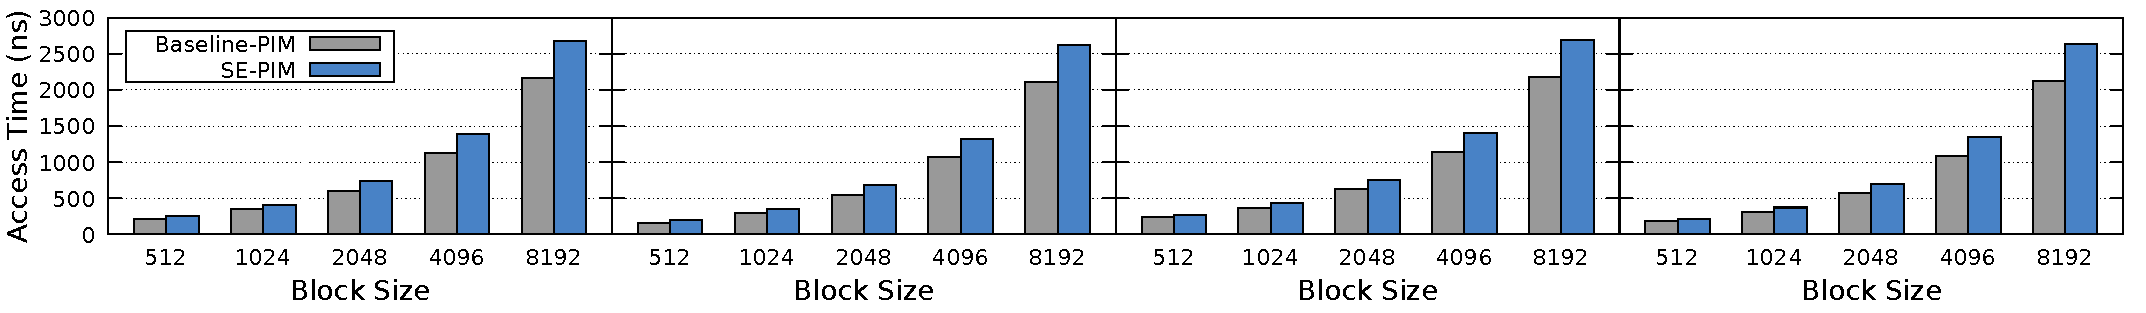
\includegraphics[width=0.95\linewidth]{figures/sepim/pim-microbenchs.pdf}
  \begin{subfigure}{.23\textwidth}
  \caption{Sequential read}
    \end{subfigure}%
  \begin{subfigure}{.23\textwidth}
  \centering
%   \includegraphics[width=0.95\linewidth]{data/gnuplot/pim-seq-write.pdf}
  \caption{Sequential write}
    \end{subfigure}%
  \begin{subfigure}{.23\textwidth}
  \centering
%   \includegraphics[width=0.95\linewidth]{data/gnuplot/pim-rand-read.pdf}
  \caption{Random read}
\end{subfigure}%
  \begin{subfigure}{.23\textwidth}
  \centering
%   \includegraphics[width=0.95\linewidth]{data/gnuplot/pim-rand-write.pdf}
  \caption{Random write}
\end{subfigure}%
\caption{Access latency of AES-encrypted DMA from bank memory to PIM local memory of \thename vs. Baseline-PIM without encryption.}
\label{fig:dma-latency}
\end{figure*}

The original attack from~\cite{membuster} requires that the host enclave caches are constantly flushed to yield reliable and distinct access patterns on the bus. We adapted the same premise for our experiment. However, since the gem5 x86 CPU model does not correctly simulate the cache flush instructions (e.g., \texttt{clflush}), we implemented a function that forces cache flush by repetitive memory accesses and used it after each hash table access to preventing caching. In the host-only setup, which represents a case where the host processor enclave is used to protect the hash table, we place the hash table inside a single memory page so that it is contiguous in physical memory. Then, we obtain the virtual to physical mapping of the program from \texttt{/proc/\{process pid\}/pagemap}. For the PIM-assisted version of the program, the hash table is stored in the PIM memory bank, and a PIM kernel that performs hash table lookups is loaded into the PIM processor local memory. We leverage our simulation framework to place a memory tracing unit between the L2 cache and DRAM (i.e., the memory bus) to collect the accessed physical addresses. \autoref{fig:access-pattern} illustrates the memory access pattern observed on the bus -- by the attacker who is snooping on the bus traffic -- in host processor execution and \thename-assisted execution.
\autoref{fig:host-pattern} shows the memory access pattern recorded during the execution of the host-only version of the test program, and \autoref{fig:pim-pattern} shows that of the \thename-assisted version (\texttt{psearch()}). The memory writes are denoted by \textcolor{blue}{$\bullet$} and reads by \textcolor{blue}{$\circ$}. 

\hdr{Results.} 
%\hjc{If you are going to use this hdr, do it for all experiments}
In the CPU-only version, the executed function and the words looked up in the hash tables are observable to the adversary. With the assumption that the adversary has the pre-obtained knowledge on the addresses of the functions and data of the program, the adversary learns that \texttt{search()} has been executed and in-memory dictionary locations, such as \texttt{hashtable[7]}, \texttt{hashtable[237]}  are accessed. As a result, the adversary can eventually infer the queried words by looking at the bus traffic. On the other hand, the PIM-assisted version shows only the communication with PIM. The PIM command channel and parameter channel are fixed single-channel memory-mapped I/O channels. The host program first writes the parameter (e.g., \texttt{"apple"} to the parameter channel, then writes the command number that corresponds to the PIM function \texttt{search()} in the PIM kernel to the command channel to invoke the offloaded task. These patterns are identical to all PIM kernel invocation, regardless of the invoked function and parameters. Also, data access (e.g., the hash table in this example) is contained inside the DRAM package. This example clearly shows the security advantages of \thename against side-channel attacks that target the bus traffic. We further discuss the security of \thename in a more comprehensive manner in \cref{sec:discussion}.






\subsection{Microbenchmarks}
\label{subsect:aes-dma}
\label{subsec:microbench}
We measure the performance of encrypted DMA transfer and the secure memory access interface with our microbenchmarks. The results suggest that encrypted DMA transfer would incur only minor overhead in each transfer, and the throughput of the controlled memory access channel would scale with the transfer size.

%Second, we measure the throughput of the memory accesses performed by host enclave through the secure access interface (explained in \cref{subsec:secure-access}). 

% We measure the performance of two operations, the encrypted data movement between PIM local memory and the memory bank, and


% Encrypted data movement is the fundamental building block of \thename design. PIM core accesses data in the memory bank by decrypting and moving the encrypted data into its local memory. . We evaluated the performance of encrypted data movement using \thename simulation to measure its performance. In the experiment, the access times and throughput of AES-enabled DMA transfers in a single \pimenclave are measured and compared with the baseline PIM simulation model, which we shall call \emph{PIM-Baseline}, that does not support any cryptographic protection for DMA transfers.







\subsubsection{Encrypted DMA transfers}
We evaluate the overhead of encrypted data movement between PIM local memory and the memory bank, when accelerated by the hardware AES engine. The average throughput of the operation is also evaluated. For both PIM-baseline and \thename, we measured the access time for the following cases: 1. in both directions (local-to-bank and bank-to-local), 2. sequential and random accesses and 3. for varying block sizes.

\hdr{Results.}  \autoref{fig:dma-latency} illustrates the average access time measured for $1000$ DMA accesses in each configuration. The access time for random and sequential access is roughly similar because there is no cache on PIM that incurs variations in access time. Our simulation results report an average of $22.35$\% of increase in access time due to the AES-capable DMA engine. This is in line with the previous works that simulated the performance overhead of hardware AES support, such as~\cite{obfusmem,invisimem}. 

We further investigated the throughput for data transfer between the memory bank and local memory. The DMA maximum throughput of moving data with the AES-capable DMA engine is compared to that of without encryption in PIM-Baseline. Overall, the AES-enabled DMA engine produces an average throughput of $2.9$ GB/s, compared to $3.53$ GB/s for unencrypted DMA accesses.
\begin{figure}[t]
    \centering
    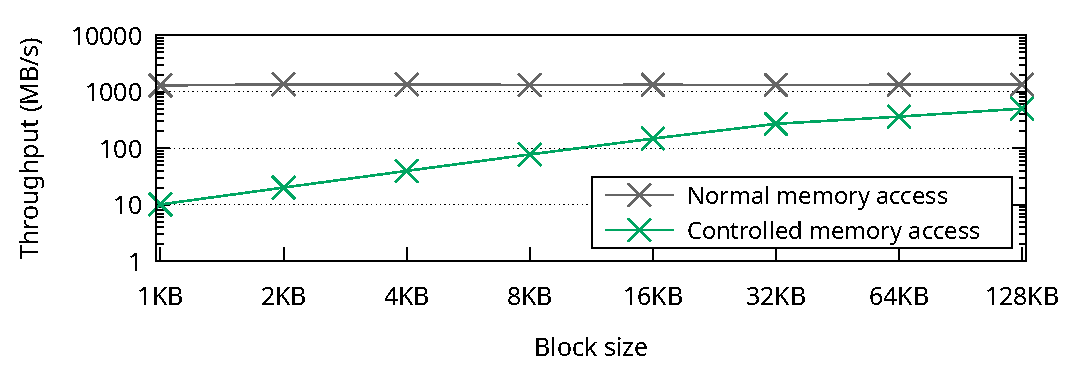
\includegraphics[width=.80\textwidth]{figures/sepim/secure-interface-throughput.pdf}
    \caption{The throughput of the controlled memory access channel on different block sizes in log-scale.}
    \label{fig:secure-access-throughput}
\end{figure}


\subsubsection{Controlled data access throughput}
\label{subsec:secure-access-eval}
We measure the throughput of data access performed through the controlled data channel (\cref{subsec:secure-access}) and compare it to the throughput of normal DRAM access to the memory. The throughput of different block sizes are measured. 



\hdr{Results.} \autoref{fig:secure-access-throughput} illustrates the results of the evaluation. Only read accesses are shown, since the performance of read and write accesses is almost identical. The results show that when small block sizes are used, a large proportion of the overhead comes from the communication channels (e.g., the MMIO accesses for writing commands), which significantly degrade the throughput of the controlled memory access channel. For instance, the throughput of $1$ KB block accesses is $127\times$ lower than normal memory accesses. However, the throughput is significantly higher when larger block sizes are used, $362.7$ MB/s for $64$ KB blocks and $504.2$ MB/s for $128$ KB blocks. The throughput of normal memory access is roughly the same among different block sizes, about $1300$ MB/s.
Despite having a lower throughput than direct memory access, the interface is faster than most ORAM implementations, which include expensive reshuffling operations at each memory access~\cite{zerotrace}. Since most of the data is already placed inside memory for PIM computation, we expect the controlled memory accesses not to be a bottleneck in PIM workloads.



%the interface would not become a bottleneck for \thename applications, since most PIM workloads reuse data within the memory bank.
%Since for most PIM workloads, data mostly stays inside memory 


% General algorithm

% \begin{figure}[b]
%   \setlength{\belowcaptionskip}{-10pt}
%   \centering
%   \includegraphics[trim=0 0 0 0,width=\linewidth]{images/bandwidth.eps}
%   \caption{Peak throughput for DMA transfers}
%   \label{fig:dma-bandwidth}
% \end{figure}



% \begin{figure}[b]
%     \centering
%     \includegraphics[width=.8\columnwidth]{images/k-mean.pdf}
%     \caption{The simplified diagram of $k$-mean clustering algorithm between host and \thename. The host send the parameters, including the current global clusters (e.g., $x_G, y_G, z_G$) to command \pimenclaves to start execution. On each \pimenclave, the kernel loop through the data points stored in the memory bank and update the local clusters (e.g., $x_L, y_L, z_L$), until all data points are processed. Then, the \pimenclave send the updated cluster, along with the \emph{delta} value to the host. The host uses information aggregated from \pimenclaves to update the global cluster, then start another round of $k$-mean if needed. }
%     \label{fig:kmean}
% \end{figure}
% \fix{This can be general PIM-enclave computation model? does it need to be a dedicated figure for k-mean?}

\begin{figure*}[t]
%   \setlength{\belowcaptionskip}{-10pt}
  \centering
  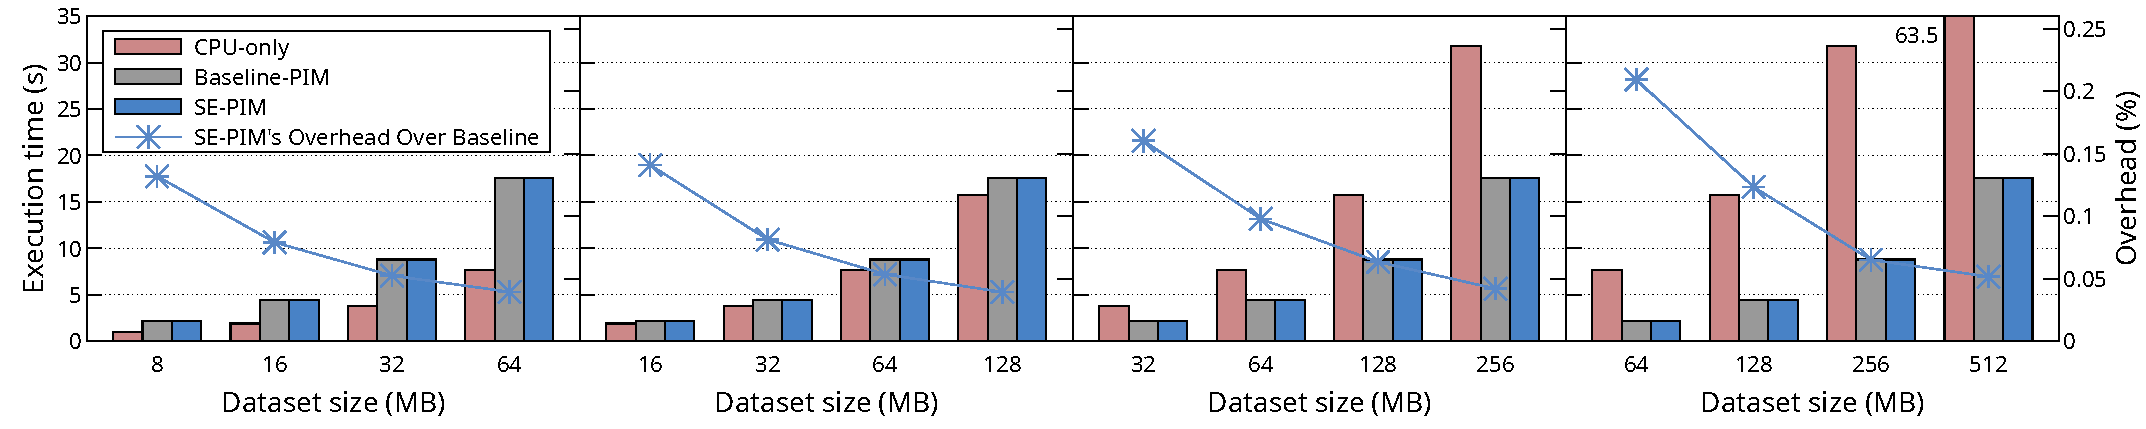
\includegraphics[width=0.95\textwidth]{figures/sepim/kmean-performance.pdf}
    \begin{subfigure}{.23\textwidth}
  \caption{1 PIM Core}
    \end{subfigure}%
  \begin{subfigure}{.23\textwidth}
  \centering
%   \includegraphics[width=0.95\linewidth]{data/gnuplot/pim-seq-write.pdf}
  \caption{2 PIM Cores}
    \end{subfigure}%
  \begin{subfigure}{.23\textwidth}
  \centering
%   \includegraphics[width=0.95\linewidth]{data/gnuplot/pim-rand-read.pdf}
  \caption{4 PIM cores}
\end{subfigure}%
  \begin{subfigure}{.23\textwidth}
  \centering
%   \includegraphics[width=0.95\linewidth]{data/gnuplot/pim-rand-write.pdf}
  \caption{8 PIM Cores}
\end{subfigure}%
  \caption{The execution time of confidential k-mean using \thename against the baseline PIM and CPU-only versions (without data encryption). \thename overhead over the baseline PIM and the performance numbers of using different numbers of PIM cores are measured.}
  \label{fig:kmean-perf-versus-baseline}
\end{figure*}

\subsection{Protected Data-intensive Computation Performance}
 
\label{subsec:app-perf}
\label{subsec:kmean}
% \input{figures/k-mean}
% \new{We developed a proof-of-concept application to evaluate the performance in data-intensive applications and the feasibility of the programming model. We choose $k$-mean as a representative application, because ... . First, it does not require frequent direct data access. Second, the computation can be distribute onto multiple \pimenclaves, which highlight the performance characteristics of PIM~\cite{upmem-atc}}
% \wip


To evaluate the performance of \thename on real-world workloads, we implement a confidential k-mean clustering application powered with \thename and compare its performance with an implementation on the baseline PIM. 
k-mean clustering is a standard algorithm in data analytics that aggregates data points into clusters. The application requires a large amount of data movement, making it a prime candidate for PIM-based accelerator~\cite{dual,prins}. 
In our confidential k-mean clustering, the adversary observing the computation learns no information about the computation. Moreover, our system allows the host enclaves to process data larger than the memory limitation of SGX-based enclaves ($96$ MB). When 8 \thename-enabled memory banks are used, up to $512$ MB of data can be processed concurrently. As more \thename units are employed, more data can be processed. 

%The algorithm starts by selecting a group of $k$ coordinates as the \emph{centroids} of the initial clusters, then iteratively updates the centroids of clusters in two steps. First, it \emph{assign} every data point to their nearest cluster, i.e., the cluster that has the smallest \emph{Euclidean distance} to the data point. Then, it \emph{update} the centroids by finding the mean of data points that belong to a cluster.

% \hdr{Evaluation objective. }



% In our $k$-mean implementation, we offload the core algorithm that incurs frequent memory access to \thename. The host distributes the encrypted data into multiple \thename memory banks, sends commands and parameters to \thename PIMs to initiate computation, then collects and aggregates the results into new \emph{global centroids}.  Upon receiving the command, the $k$-mean PIM kernel is executed in response. The kernel finds \emph{pointer} to the data to be computed in the DMA buffer along with other parameters. 
% How it is implemented as PIM kernel and PIM-enclave specific programming model

% \hdr{Advantages of \thename-assisted k-mean clustering.}
% The k-mean algorithm on \thename demonstrates our capabilities as a large data accelerator and secure storage by the host. In the algorithm, no data movement occurs between the host enclave and PIM between each kernel execution. Instead, only the arguments for the kernel execution, which includes the pointer of data, the size, the initial clusters, are sent from the host enclave to PIM. After a PIM kernel finishes its execution, only computation results are sent back to the host enclave through the secure channel. The elimination of data movement has two significant implications. First, efficiency was achieved in terms of the total execution time of the particular task and memory bus bandwidth usage. Second, the computation did not leave any pattern on the memory bus. This is only possible on PIM-based computation since CPUs, or any accelerators on the peripheral bus, inevitably access memory with patterns unless using ORAM primitives. With DRAM lockdown, our system also eliminates the access pattern leaked by the memory content changes from data update of the membership data~(\cref{subsec:access-control}).

% \thename also function as a secure memory extension for the host enclave. After data have been loaded into the \pimenclaves, the host enclave need not keep the data inside its EPC memory. Our secure memory access interface described in \cref{subsec:secure-access} hides the address side-channel in cases where host-side data accesses are required. Moreover, the more of \thename units are employed, the more data the host enclave can process and use without EPC swapping. This allows us to overcome the memory limitations of CPU-based secure enclaves.

\hdr{Implementation details.} 
We implement k-mean clustering to perform the data aggregation part on \thename and the baseline PIM. A dataset of randomly generated data points with $16$ different coordinates is used. We preprocess the dataset by partitioning data coordinates into $8$ KB blocks. For the \thename version of k-mean, we encrypt batches of data into encrypted blocks. For each data block, we also use a structure to store the \emph{membership data} (e.g., which cluster the objects belong to) of objects in the block and load them along with the objects into the memory bank. When multiple PIM cores are utilized, data is distributed evenly among the memory banks of different PIM cores. We then create a CPU thread for each PIM core to launch the PIM kernel and wait for the results. The host use the \emph{local clusters} aggregated from different PIM banks to update the \emph{global clusters}.

We implement the PIM kernel to perform k-mean aggregation on data inside the memory bank in a batch of $127$ objects at a time. Each processing batch fetches the objects and their membership data inside the bank memory into local memory. First, it assigns every data point to its nearest cluster, i.e., the cluster that has the smallest \emph{Euclidean distance} to the data point. Then, it recalculates the local clusters of data points inside the memory bank. Finally, the kernel encrypts updates the new membership data into memory before moving on to the next batch. In the version of k-mean powered by \thename, data movement between the local memory and the memory banks is automatically encrypted/decrypted by the AES-capable DMA engine (\cref{subsec:aes-dma}). After all data in the memory bank has been processed, the kernel sends the results (the local clusters and additional metadata) to the host.





\hdr{Results. }
\autoref{fig:kmean-perf-versus-baseline} demonstrates the performance of executing a round of k-mean on \thename in comparison to executing the same algorithm on the baseline PIM. For PIM-based scenarios, we repeat the experiment until the maximum capacity of the PIM-enabled memory banks is reached. When 8 PIM cores are used, the maximum size of the data set is $512$ MB, which corresponds to $80,000,000$  data points. We also measure the algorithm's performance on the CPU (without PIM assistance) on similar data sizes for comparison. The specification of the CPU is described in \autoref{table:config}.

The simulation results support that using that \thename as an accelerator for large data secure computation is efficient. 
The total runtime of \thename's confidential k-mean on encrypted data has negligible overhead to the baseline model without encryption. The results also show that as the data set sizes increase, the overhead of \thename over \baseline also decreases. On average, the execution time of the confidential k-mean algorithm incurs $0.075$\%, $0.079$\%, $0.09$\%, $0.11$\% overhead compared to the insecure version when 1, 2, 4, and 8 PIM cores are used, respectively. Moreover, our system attains speed up in execution time compared to performing k-mean only with the CPU. \thename outperforms the CPU-only k-mean when more than 4 PIM cores are used. When processing $512$ MB of data with 8 PIM cores, \thename achieves $3.61 \times$ speed up to just using the CPU, with the execution time of $17.6$ seconds ($0.05$\% more than the baseline-PIM version). Note that the application's execution time on the CPU is optimistic in our evaluation. We do not consider the overhead of EPC swapping due to extensive memory usage, which can incur up to $1000\times$ performance degradation in some applications~\cite{zerotrace,scone}.


% Moreover, the performance of \thename's k-mean scales with the number of PIM cores. This is  %We use increasing dataset sizes up to $64$ MB, which corresponds to $10,000,000$ data points. % When only $4$ \thename PIM devices are deployed, the execution time of $k$-mean is below that of the host on the same amount of data, with $21.7\%$ performance degradation. The reason is that there is a bottleneck in the communication between the host and PIM. However, \thename outperformed the execution time of the host with more than six \thename-enabled PIMs.
\section{Security Analysis and Discussion}
\label{sec:sec-analysis}
\label{sec:discussion}



\begin{table}[t]
    \scriptsize
	\renewcommand{\arraystretch}{0.8}
	\renewcommand{\theadgape}{\Gape[.2pt]}
	
    \centering
  	\renewcommand\theadfont{\bfseries}
    \begin{tabular}{p{5.8cm}p{7.5cm}}
        \toprule
        \thead{Attack Vector} & \thead{Mitigation}\\
        % \midrule
        % CPU-side side-channels & Offload the computation to \thename\\ 
        \midrule
        \makecell[l]{Capturing and tampering of host-\thename \\communication, unauthorized \thename\\ commands, side-channels and replaying\\ of messages}& Secure channel protected by authenticated encryption~(\cref{subsec:attestation})\\ 
        \midrule
        Address side-channel on bus from host-side memory accesses(\challenge{2}) & Controlled memory access channel~(\cref{subsec:secure-access})\\ 
        \midrule
        \makecell[l]{Memory content change side-channel (\challenge{3}), \\  encrypted data modification (\challenge{4})} & \makecell[l]{DRAM lockdown unit~(\cref{subsec:access-control})}\\ 
       \midrule
        Cold boot attacks & Maintaining encrypted bank memory and only keep decrypted data in the protected local memory (\cref{subsec:aes-dma}) \\ 
    
        \bottomrule
    \end{tabular}
    \caption{Attack Vectors on \thename's confidential computation and mitigations.}
    \label{tab:sec-analysis}
\end{table}

% \subsection{Security analysis}
In this section, we provide a security analysis of our proposed solution. Apart from the imperative features for confidential computation, we also propose solutions for each of the challenges identified in \cref{subsec:challenges}. \autoref{tab:sec-analysis} summarizes the attack vectors and our proposed mitigation in \thename. We also discuss the potential side-channel within a \thename-enabled memory module. 

%\hdr{Secure communication channel.} 


\subsection{Address side-channel on bus} An attacker with physical access that snoops on the memory bus will only see the commands sent to \thename from the host enclave and the encrypted parameters. This is further confirmed in our memory access pattern evaluation shown in~\cref{subsect:memory-access-pattern}. With the introduction of remote attestation capabilities and secure channel establishment (\cref{subsec:attestation}), \thename can build a secure communication channel between the host enclave and the assisting \thename unit. Standard techniques are employed to secure the channels against tampering and side-channel. An increasing counter is used to prevent the replaying of messages. We also use fix-sized messages to thwart side channels from different message sizes. \thename also prevents unauthorized commands by using authenticated encryption. Our programming model moves the sensitive operations into memory, eliminating the memory access pattern shown on the bus.  With our controlled access channel (described in~\cref{subsec:secure-access}), memory accesses from the host enclave are also resistant against the address side-channels.

\subsection{Unauthorized memory accesses and cold boot attacks} Our DRAM lockdown unit (\cref{subsec:access-control}) deny accesses to \thename-protected data during PIM computation. This brings two advantages. First, unauthorized system software (e.g., the kernel) or malicious DMA devices cannot capture memory snapshots and extract the memory content changes. Second, adversaries cannot modify the memory content to perform splicing and replaying attacks.
On the other hand, our design choice was to keep the data residing in the memory bank encrypted, even with the new capability to drop access to the memory bank. An adversary with physical access to the memory module may launch a cold boot attack to dump the memory contents in the memory bank but can only obtain encrypted values. This guarantees the confidentiality of data protected by \thename.


\subsection{Potential side-channels inside memory module}
In our current design, a \thename-enabled memory module can support multiple users by allowing the remote user to establish trust with each \thename unit independently (e.g., through PIM attestation). Only one host enclave can establish a secure channel and use a \thename unit in a single session.
Moreover, there is no communication or shared resources among the memory banks inside \thename-enabled memory modules. A PIM core can only access its local memory and bank memory (i.e., it cannot access other bank memory). Hence, no hardware connections can be exploited to create side channels between PIM cores. Such strict separation prevents security risks from malicious co-tenants who have access to one or more \thename banks. Being the first to explore confidential computing inside PIMs, our design focuses on maintaining the confidentiality of the computation. We expect that secure communication between PIM banks can enable more flexible forms of computation inside PIM~\cite{tesseract}. 


\section{Conclusion}
We presented \thename, an architecture that enables confidential computing inside memory by retrofitting the processor-in-memory architecture. Through a careful security analysis of the new architecture, we proposed a set of non-intrusive yet imperative changes that guarantees the data's confidentiality and integrity computed inside PIM. We evaluated our design and a proof-of-concept application for our design using a cycle-accurate full-system simulation. Our evaluation shows that the encrypted data transfer in our design only incurs a $17.85\%$ overhead in the maximum throughput inside memory compared to the unmodified PIM architecture that does not support encryption. We also evaluated a confidential k-mean program that runs on our architecture to accelerate data-intensive operations. We observed only $0.05$\% increase in total execution time on the most significant data size compared to offloading to the unprotected PIM architecture. 


